\documentclass[11pt, a4paper, twoside, openright]{book} 
\usepackage[italian, english]{babel}
\usepackage[sc]{mathpazo}
\usepackage[utf8]{inputenc}
\usepackage{setspace}
\onehalfspacing	
\usepackage{microtype}
\usepackage[inner=4cm, outer=3cm, top=3cm, bottom=3cm]{geometry}
\usepackage{graphicx}
\graphicspath{ {./img/} }
\usepackage{tabularx}
\usepackage{booktabs}
\usepackage[hang, small,labelfont=bf,up,textfont=it,up]{caption}
\usepackage[Bjornstrup]{fncychap}
\ChNumVar{\fontsize{76}{80}\usefont{OT1}{pzc}{m}{n}\selectfont\color{black}}  
\ChTitleVar{\raggedleft\LARGE\bfseries}
\usepackage{epigraph}
\usepackage{xcolor}
\usepackage{multicol}
\usepackage{pdfpages}
\usepackage[pdftex]{hyperref}
\hypersetup{
	bookmarksnumbered,	% Chapter and Appendix Numbers
	colorlinks,
	citecolor=black,
	filecolor=black,
	linkcolor=black,
	urlcolor=black
}
\usepackage{listings}
\usepackage{multicol}

\definecolor{backcolour}{RGB}{255,255,255}
\definecolor{codegreen}{RGB}{27,168,11}
\definecolor{codeblue}{RGB}{35,35,205}
\definecolor{codegray}{RGB}{128,128,128}
\definecolor{codepurple}{RGB}{205,35,56}
\lstdefinestyle{myPython}{
	backgroundcolor=\color{backcolour},   
	commentstyle=\color{codegreen},
	keywordstyle=\color{codeblue},
	numberstyle=\tiny\color{codegray},
	stringstyle=\color{codepurple},
	basicstyle=\small\ttfamily,
	breakatwhitespace=false,         
	breaklines=true,                 
	captionpos=b,                    
	keepspaces=true,                 
	numbers=left,                    
	numbersep=5pt,                  
	showspaces=false,                
	showstringspaces=false,
	showtabs=false,                  
	tabsize=2,
	language=python
}

\usepackage[titletoc]{appendix}

\title{Tesi Triennale}
\author{FEDERICO MATTEONI}
\date{Giugno-Agosto 2021}

\begin{document}
	\selectlanguage{italian} 
	
	\frontmatter
	% Il frontespizio viene importato da un file pdf con una singola pagina
	\begin{titlepage}
		\thispagestyle{empty}
		
\includepdf{frontespizio/frontespizio.pdf}
		\thispagestyle{empty}
		\cleardoublepage
	\end{titlepage}	
	%\null \vspace{\stretch{1}}
\begin{flushright}
\textit{Dedica per qualcuno}
\end{flushright}
\vspace{\stretch{2}} \null \cleardoublepage
	\cleardoublepage
	\phantomsection
	\pdfbookmark{\contentsname}{tableofcontents}
	\tableofcontents
	\cleardoublepage
	\phantomsection
	\addcontentsline{toc}{chapter}{Immagini}
	\listoffigures
	\cleardoublepage
	\phantomsection
	\addcontentsline{toc}{chapter}{Tabelle}
	\listoftables
	\phantomsection
\chapter*{Glossario}
\markboth{GLOSSARIO}{}
\addcontentsline{toc}{chapter}{Glossario}

\subsection*{Abbreviazioni e Acronimi}
\begin{table}[h!]
	\begin{center}
		\begin{tabularx}{\textwidth}{ll}
			\toprule
			\textsc{Termine} & \textsc{Significato} \\ 
			ML & Machine Learning\\
			HSM & Human State Monitoring, Monitoraggio dello Stato Umano\\
			ReLU & Rectified Linear Unit, Unità Lineare Rettificata\\
			RNN & Recurrent Neural Network, Rete Neurale Ricorrente\\
			LSTM & Long Short-Term Memory, Memorie a Lungo Breve-Termine\\
			LWF & Learning Without Forgetting, Apprendere Senza Dimenticare\\
			EWC & Elastic Weight Consolidation, Consolidamento Elastico dei Pesi\\
			FWT & Forward Transfer, Trasferimento in Avanti\\
			BWT & Backward Transfer, Traserimento all'Indietro\\
			HAR & Human Activity Recognition\\
			MNIST & Modified National Institute of Standards and Technology Database\\
			GRU & Gated Recurrent Unit, Unità Ricorrente con Cancello\\  % intraducibile
			GPU & Graphics Processing Unit, Unità di Processo Grafico\\
			TPU & Tensor Processing Unit, Unità di Processo Tensoriale\\
		\end{tabularx}
	\end{center}
\end{table}
	\phantomsection
\chapter*{Introduzione}
\markboth{INTRODUZIONE}{}
\addcontentsline{toc}{chapter}{Introduzione}

Negli ultimi decenni, le "intelligenze artificiali" si sono fatte sempre più spazio nella nostra vita di tutti i giorni. Grazie ai nostri smartphone, usiamo modelli di machine learning ultra efficienti che indirizzano le nostre ricerche nella rete, e grazie a tali modelli le aziende possono mostrarci inserzioni sempre più aderenti ai nostri gusti personali. Ma il mondo del machine learning ha importanti e utili applicazioni anche nella salvaguardia del benessere dell'individuo, ad esempio in contesti come il riconoscimento delle malattie o l'interpretazione del linguaggio parlato.

\subsection*{Human State Monitoring}
Uno di questi contesti è lo \textit{Human State Monitoring}. Con questo termine si indica l'obiettivo di un sistema di raccogliere dati riguardanti l'attuale stato psico-fisico di un individuo e trarre conclusioni sulla sua condizione attuale, ad esempio interpretando un battito cardiaco elevato insieme ad un alto livello di sudorazione come uno stato di stress, o determinati movimenti facciali come una condizione di sonnolenza. L'avere a disposizione metodi efficienti nel catalogare queste condizioni umane può portare a sistemi responsivi e adattivi, che modificano le proprie interfacce o i propri comportamenti accomodando lo stato psico-fisico attuale dell'utente.\\\\
Un esempio di questa applicazione lo si può trovare nel progetto europeo\\TEACHING$^{\cite{teaching2020}}$, che mira alla produzione di un toolkit per costruire applicazioni autonome efficienti che facciano uso di intelligenza simile a quella umana. L'obiettivo di questo toolkit è supportare lo sviluppo e il rilascio di applicazioni che possano sfruttare il feedback umano per ottimizzare, personalizzare e guidare il modo in cui esse forniscono i propri servizi. In altre parole, applicazioni che sfruttino lo \textit{Human State Monitoring} per adattarsi dinamicamente alle condizioni dell'utente in tempo reale.\\
Per poter realizzare questo continuo adattamento è necessario, oltre al flusso di dati in tempo reale sullo stato corrente dell'utente, anche un sistema che sappia efficientemente e correttamente interpretare questi dati e trarre conclusioni sulle attuali condizioni della persona. Questa situazione rispetta le classiche caratteristiche necessarie all'applicazione del machine learning: abbiamo dati raccolti da sensori che possono essere difettosi, per cui i dati possono contenere incertezze o essere rumorosi o incompleti, ed essendo in esame lo stato umano è molto difficile, se non impossibile, formalizzare attraverso una serie di formule la classificazione di questi dati in categorie comportamentali come affaticamento o sonnolenza.

% breve introduzione al mondo dell'addestramento machine learning per introdurre i concetti fondamentali per la tesi
\subsection*{Addestramento} L'addestramento supervisionato di un modello di machine learning avviene attraverso l'utilizzo di un insieme di dati chiamato \textit{training set}. Questo insieme contiene dati a cui è stata assegnata un'etichetta, e si contrappone all'apprendimento non supervisionato dove ai dati di addestramento non è assegnata alcuna etichetta. Nel nostro caso, prenderemo in considerazione l'apprendimento supervisionato.\\
Il modello di machine learning, attraverso una serie di algoritmi, elabora questi dati e le loro etichette cercando di apprendere quali etichette sono assegnate a quali dati. Per verificare l'apprendimento, si sottopone al modello addestrato dei dati non etichettati, denominati \textit{test set}, e si verificano le etichette che il modello assegna a tali dati controllando se ha classificato correttamente o meno. La percentuale di classificazioni corrette è chiamata \textbf{accuratezza} del modello.

\subsection*{Loss} Per misurare l'andamento dell'apprendimento di un modello di machine learning, vengono usate funzioni che vanno a valutare il modello in base alle risposte che fornisce sui dati etichettati, confrontandole con le etichette vere. Queste funzioni prendono il nome di funzioni di \textit{loss}, e ne esistono di diversi tipi a seconda del problema in esame: ad esempio, nei problemi dove ad ogni input va assegnata una risposta si/no (classificazione binaria) una loss molto usata è la cross-entropia binaria (\textit{binary crossentropy}).

\subsection*{Reti Neurali} In letteratura vengono studiati moltissimi modelli di machine learning. Si va dai più semplici come i modelli lineari, nei quali abbiamo un'equazione nella forma $y = w_0x + w_1$ e dobbiamo apprendere i $w_0$ e $w_1$ che ai dati $x$ fanno corrispondere le corrette etichette $y$, alle \textit{Support Vector Machine}, che cercano di trovare dei confini di divisione fra insiemi di dati in modo da classificarli.\\
Un'ampia area di modelli di machine learning è quella delle cosiddette \textbf{reti neurali}, studiate sin dagli anni '40. Esse prendono liberamente spunto dalla struttura dei neuroni del cervello umano (Figura \ref{fig:neurone}), che sono stati schematizzati in strutture matematiche denominate \textbf{perceptron}.
\begin{figure}[h]
	\begin{center}
		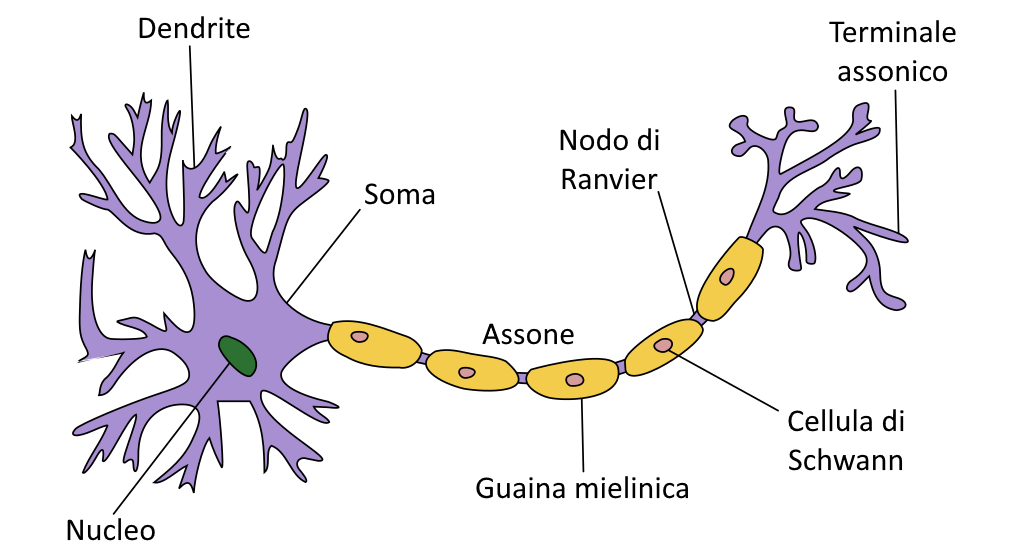
\includegraphics[width=0.75\textwidth]{img/neurone.png}
		\caption{Neurone (credits: Quasar, Wikipedia)}
		\label{fig:neurone}
	\end{center}
\end{figure}
In un perceptron (Figura \ref{fig:perceptron}), ad ogni input $x_i$ è assegnato un peso $w_i$ che lo rende più o meno importante nel contribuire al risultato $y$, che viene calcolato dal nodo attraverso la \textbf{funzione di attivazione}.\\\\
\begin{figure}[h]
	\begin{center}
		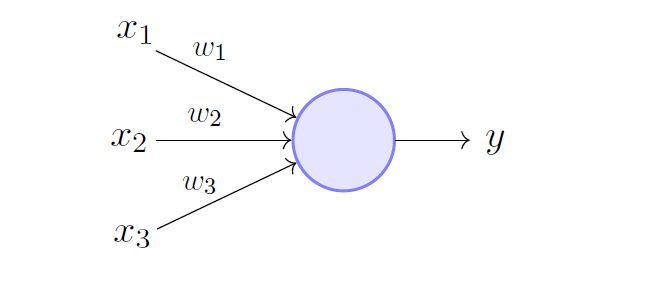
\includegraphics[width=0.5\textwidth]{img/perceptron.png}
		\caption{Perceptron}
		\label{fig:perceptron}
	\end{center}
\end{figure}
Una rete neurale (Figura \ref{fig:reteneurale}) è composta da un insieme di perceptron collegati fra loro suddivisi su livelli, o \textit{layer}: una rete neurale composta da un elevato numero di layer è detta profonda, o \textit{deep neural network}, e i layer interni sono detti layer nascosti.
\begin{figure}[b]
	\begin{center}
		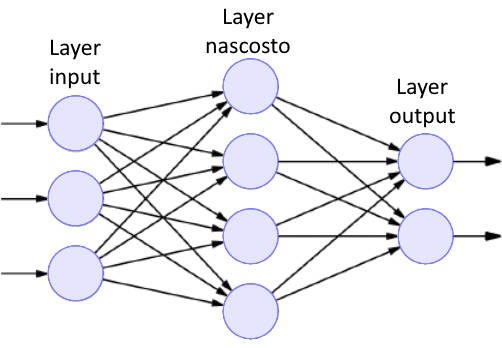
\includegraphics[width=0.75\textwidth]{img/reteneurale.jpg}
		\caption{Esempio di rete neurale}
		\label{fig:reteneurale}
	\end{center}
\end{figure}
\\\\
Le funzioni di attivazione possono essere funzioni di qualsiasi tipo, ma le più usate e studiate sono funzioni specifiche come ReLU e softmax. La funzione ReLU (\textit{Rectified Linear Unit}) è molto semplice e veloce da calcolare: restituisce la parte positiva del proprio input, e consente un migliore apprendimento nelle reti neurali profonde$^{\cite{pmlr-v15-glorot11a}}$.
\begin{equation}\label{eq:fun_relu}
ReLU(x) = max(0, x)
\end{equation}
La funzione softmax, invece, prende in input un vettore di $K$ valori e lo comprime in un vettore sempre di $K$ valori ma compresi in un intervallo $(0, 1)$ e la cui somma è 1. Vengono usate nel layer finale delle reti neurali classificatrici: ogni valore $\sigma(\textbf{z})_j$  è interpretabile come la probabilità che l'input appartenga ala classe $j$ fra le $K$ possibili.
\begin{equation}\label{eq:fun_softmax}
\sigma(\textbf{z})_j = \frac{e^{z_j}}{\sum_{k=1}^K e^{z_k}}\:\:\:\:per\:\:j = 1,\ldots,K
\end{equation}
Le funzioni di attivazione descrivono quindi il comportamento dei nodi di una rete neurale e la scelta della funzione di attivazione è un elemento importante nella strutturazione di una rete neurale. Abbiamo fatto l'esempio di ReLU, tipicamente usata nei layer nascosti, e di softmax, usata nei layer di output, ma ce ne sono molte altre adatte per altri problemi.
\subsection*{Tipologie} La struttura interna di una rete neurale influenza particolarmente i risultati che essa può ottenere. A seconda del problema che si vuole risolvere, si può avere bisogno di reti neurali con strutture interne più complesse per ottenere risultati apprezzabili. In particolare, in letteratura attualmente alcune delle strutture più studiate sono (Figura \ref{fig:tipologiereti}):
\begin{itemize}
    \item[-] Reti Feed Forward (FF)
    \item[-] Reti Neurali Ricorrenti (RNN, Recurrent Neural Networks)
    \item[-] Auto Encoders (AE)
    \item[-] Reti Profonde Convolutive (DCN, Deep Convolutional Networks)
    \item[-] Echo State Networks (ESN)
\end{itemize}
e moltissime altre. Alcune strutture sono particolarmente usate su certe tipologie di problemi: ad esempio, le DCN hanno una struttura ispirata alla corteccia visiva animale e sono particolarmente usate nel campo del riconoscimento delle immagini e del linguaggio parlato, mentre le RNN mantengono informazioni riguardo gli input precedenti e consentono di modellare i comportamenti dinamici e ricorrenti delle sequenze temporali.
\begin{figure}[b]
	\begin{center}
		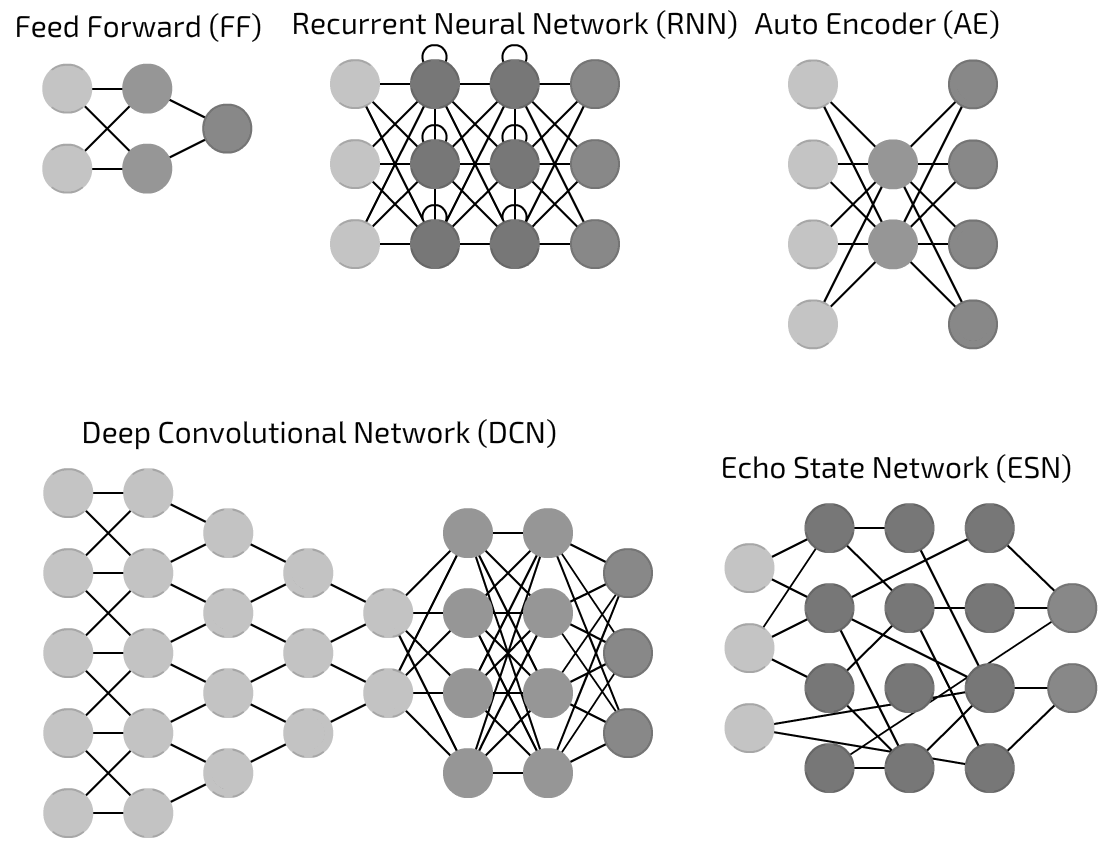
\includegraphics[width=0.95\textwidth]{img/tipologiereti.png}
		\caption{Esempi di reti neurali}
		\label{fig:tipologiereti}
	\end{center}
\end{figure}

\subsection*{Backpropagation} La retropropagazione dell'errore, \textit{backward propagation of errors}, è l'algoritmo più diffuso per l'addestramento supervisionato delle reti neurali. Questo algoritmo consiste di due fasi:
\begin{itemize}
    \item[-] \textit{Forward phase}, dove gli input vengono elaborati dalla rete neurale fino a produrre un output
    \item[-] \textit{Backward phase}, dove l'output prodotto è confrontato con la vera etichetta assegnata e, attraverso calcoli differenziali, vengono individuati i contributi all'errore di ogni nodo. Con questi contributi, attraverso un algoritmo di ottimizzazione (solitamente, la discesa di gradiente), vengono modificati i pesi delle connessione fra i nodi, partendo dai nodi output e risalendo la rete fino ai nodi input.
\end{itemize}
Questo algoritmo richiede quindi che le funzioni di attivazione dei nodi siano differenziabili, e può soffrire di un problema che prende il nome di \textit{vanishing/exploding gradient problem}, o problema della scomparsa/esplosione del gradiente. Nel dettaglio, attraverso questo algoritmo ogni parametro del modello viene modificato, durante la \textit{backward phase}, in maniera proporzionale alla derivata parziale della funzione \textit{loss} rispetto al parametro stesso. Propagando all'indietro attraverso la regola della catena$^{(\ref{eq:catena})}$ dei gradienti compresi nell'intervallo $[0, 1]$, come nel caso di alcune funzioni di attivazione, il prodotto diventa tanto più piccolo quanto più è profonda la rete neurale o, viceversa, esplodere in caso di gradienti dai valori elevati.
\begin{equation}\label{eq:catena}
D\left[f(g(x))\right] = f'(g(x))\cdot g'(x)
\end{equation}
Questo problema viene mitigato dall'uso di funzioni di attivazioni diverse, come le già citate ReLU$^{(\ref{eq:fun_relu})}$ e softmax$^{(\ref{eq:fun_softmax})}$, o dall'uso di algoritmi di addestramento che fanno uso solo del segno del gradiente e non della sua norma, come l'algoritmo Rprop$^{\cite{Riedmiller92rprop-}}$.\\
Nelle reti neurali ricorrenti, un grande contributo alla mitigazione del problema è avvenuto grazie all'introduzione delle LSTM, \textit{Long-Short Term Memory}, che mantengono informazioni sullo stato del modello senza propagarle attraverso funzioni non lineari.

\subsection*{Continual Learning} L'addestramento di un modello di machine learning attraverso un \textit{training set} disponibile fin da subito e fornito al modello tutto in una volta è denominato "addestramento \textit{offline}", o \textit{offline training}. Esistono contesti, però, dove i dati necessari o utili all'addestramento non sono subito tutti disponibili, ma diventano tali col passare del tempo. Un esempio di questa situazione sono i sistemi di raccomandazione in servizi come Netflix o YouTube: essi imparano continuamente i gusti dell'utente, in modo da fornire suggerimenti su video e film sempre adatti ai gusti del momento. Questa situazione, in cui i dati di addestramento diventano disponibili col passare del tempo e cioè di addestramento continuativo, è detta "addestramento \textit{continual}", o \textit{continual learning}.\\
Nel caso del \textit{continual learning}, un grosso ostacolo è quello denominato \textit{catastrophic forgetting}$^{\cite{MCCLOSKEY1989109}}$: quando una rete neurale già addestrata viene addestrata su nuovi dati, essa tenderà a dimenticare ciò che ha appreso sui dati precedenti. Questa situazione è una manifestazione del cosiddetto dilemma della \textbf{plasticità-stabilità}: si ha stabilità quando la nuova conoscenza non interferisce con la vecchia conoscenza, mentre la plasticità è ottenuta quando la nuova conoscenza migliora la conoscenza precedente e viceversa. Questi due obiettivi sono in contrapposizione fra loro e mantenere un buon compromesso fra i due è uno degli obiettivi chiave degli algoritmi e attuale campo di studio.\\\\
Il continual learning si rende ancora più necessario in un mondo in continua e rapida evoluzione, e apporta al machine learning un cambiamento di paradigma al pari dell'introduzione della filosofia Agile$^{\cite{agilemanifesto}}$ nel mondo dell'ingegneria del software: mentre in molti dei modelli di machine learning correnti l'addestramento è eseguito da zero e il modello viene utilizzato così com'è, con un procedimento al pari dei primi approcci "a cascata" allo sviluppo software, il continual learning fornisce a questo mondo la possibilità di produrre modelli che vengono migliorati iterativamente ogni volta che c'è bisogno senza dover addestrare un nuovo modello da zero. "Il parallelismo sta nell'equiparare i dati ai requisiti (arrivano in maniera continuativa e cambiano nel tempo) e l'addestramento alla fase di design e sviluppo, che porta al prodotto software (che nel nostro caso è la funzione di predizione realizzata dal modello di machine learning)."$^{\cite{lomonaco_2019}}$

\subsection*{Conclusione} Lo \textit{human state monitoring} è un ambiente sempre più utile e importante nella realizzazione di sistemi personalizzati che rispondono dinamicamente allo stato attuale dell'utente: un esempio può essere la riduzione della velocità di un veicolo a guida autonoma quando l'utente alla guida è in stato di sonnolenza, e quindi poco attento agli eventuali errori del veicolo.\\
Per realizzare questi modelli di machine learning si rendono necessarie reti neurali ricorrenti, poiché abbiamo a che fare con flussi di dati temporali raccolti da vari sensori posti sull'utente, che devono adattarsi in maniera continuativa all'utente attuale (nell'esempio, il proprietario del veicolo) avvalendosi quindi di tecniche di continual learning, che non soffrano del \textit{catastrophic forgetting}.\\
Si necessitano quindi di metriche per misurare nel tempo l'efficienza e la precisione di questi modelli sottoposti a continual learning, per giudicare l'applicabilità delle tecniche in esame applicate allo \textit{human state monitoring}.
    
    \mainmatter
    \chapter{Obiettivi}
In un mondo sempre più interconnesso e in rapida evoluzione, approcci statici al machine learning possono diventare impraticabili quando si tratta di produrre sistemi in grado di adattarsi dinamicamente allo stato fisico e mentale degli utenti che vi interagiscono. Inoltre, con l'ampia presenza di dispositivi in grado di raccogliere anche in tempo reale informazioni sulla condizione attuale degli utenti, diventano continuamente disponibili nuovi dati con cui perfezionare i modelli di machine learning in uso attraverso tecniche di continual learning.
\section{Stato dell'Arte}
Alcuni recenti studi nell'ambito del continual learning si sono concentrati, ad esempio, sull'applicabilità pratica e l'ideazione di un'architettura in grado di manutenere modelli di machine learning in produzione e gestire la dinamicità e i cambiamenti sui dati$^{\cite{diethe2019continual}}$, oppure in ambiti come la \textit{human activty recognition} (HAR)$^{\cite{Jha_2021}}$, cioè il riconoscimento delle attività quotidiane delle persone attraverso dei sensori, o anche l'acquisizione di informazioni dai social media per, ad esempio, gestire al meglio situazioni di crisi$^{\cite{priyanshu2021continual}}$.  % obiettivi della ricerca e degli esperimenti
    \chapter{Dataset}
Ai fini del progetto, il primo elemento necessario per poter valutare correttamente la sinergia continual learning -- Human State Monitoring sono dei dati raccolti riguardanti quest'ultimo. I dati dovrebbero provenire da più soggetti, per correttezza statistica, e riguardare diversi aspetti biometrici della persona: battito cardiaco, sudorazione, respirazione\ldots\\\\
I dataset selezionati ai fini di questa comparazione sono due, che seguono.
\section{WESAD}
Il dataset WESAD$^{\cite{10.1145/3242969.3242985}}$, acronimo di \textit{WEarable Stress and Affect Detection}, contiene dati raccolti da 15 soggetti durante uno studio effettuato in laboratorio riguardante i livelli di stress misurati tramite sensori biometrici e di movimento indossabili. Il dataset classifica questi dati in tre scale: neutralità, stress e divertimento.\\
I dispositivi usati per la raccolta dei dati sono due: uno indossato sul petto (RespiBAN) e uno indossato sul polso (Empatica E4).\\\\Il RespiBAN, indossato sul petto, raccoglie dati campionati a 700 Hz su:
\begin{itemize}
    \item[-] Elettrocardiogramma (ECG)
    \item[-] Attività elettrodermica (EDA)
    \item[-] Elettromiogramma (EMG)
    \item[-] Respirazione
    \item[-] Temperatura corporea
    \item[-] Accelerazione sui tre assi
\end{itemize}
\pagebreak
L'Empatica E4, indossato sul polso, monitora con frequenza di campionamento eterogenea:
\begin{itemize}
    \item[-] Pulsazioni (BVP), a 64Hz
    \item[-] Attività elettrodermica (EDA), a 4 Hz
    \item[-] Temperatura corporea, a 4 Hz
    \item[-] Accelerazione sui tre assi, a 32 Hz
\end{itemize}
La quantità di dati contenuti in questo dataset lo rende un ottimo strumento nell'addestramento di modelli di machine learning riguardanti l'ambiente dello HSM. Dati come le pulsazioni, la temperatura e l'elettrocardiogramma sono precisissimi indicatori biometrici dello stato psico-fisico di una persona e pertanto sono estremamente utili alle reti neurali per dedurre lo stato psico-fisico di soggetto.
\subsection{Preprocessing}
Una volta caricato il dataset, i dati sono satti concatenati e ricampionati a 32 Hz, attraverso la libreria \texttt{SciPy}. Dopodiché, l'insieme delle features è stato standardizzato ponendo media pari a 0 e deviazione standard uguale a 1, sono state sincronizzate le etichette e sono state rimosse l'etichetta 0, corrispondente alla neutralità, e le etichette 5, 6 e 7 poichè secondo le indicazioni del dataset sono corrispondenti a dati da ignorare. I dati sono poi raccolti in sottosequenze di 100 punti relativi alla stessa etichetta, corrispondenti a circa 3 secondi, e per ogni etichetta vengono estratte 100 di queste sottosequenze.\\
Dai dati viene poi estratto un test set. Questo ci lascia con un test set di 1500 elementi e un training set da 4500 elementi suddivisi come specificato nella tabella \ref{tab:splittedwesad}.
% \lstinputlisting[style=myPython, firstnumber=29, firstline=29, lastline=43]{code/wesad_data.py}

\section{ASCERTAIN }
ASCERTAIN$^{\cite{10.1145/2818346.2820736}}$, acronimo di \textit{multimodal databASe for impliCit pERsonaliTy and Affect recognitIoN}, è un dataset che raccoglie dati provenienti da 58 soggetti raccolti con sensori fisiologici commerciali e classifica le informazioni su diverse scale: incitamento, valenza, investimento, apprezzamento e familiarità. Il dataset contiene anche dati relativi all'attività facciale dei soggetti registrati con sensori comuni, oltre ai dati sull'elettroencefalogramma (EEG), elettrocardiogramma (ECG) e sulle risposte galvaniche della pelle (GSR).\\\\
Il motivo principale per cui è stato selezionato ASCERTAIN sono i dati sui movimenti facciali dei soggetti. In contesti reali, dove non sempre è possibile raccogliere dati sull'utente mediante sensori biometrici applicati sul corpo del soggetto, spesso è disponibile solamente una o più videocamere che lo riprendono. Poter sfruttare questi dati non invasivi per poter trarre conclusioni relative allo HSM può rivelarsi quindi molto utile durante applicazioni reali.
\subsection{Preprocessing}
Dal dataset sono stati esclusi due soggetti poiché i loro dati risultavano imprecisi o incompleti. Ogni soggetto è stato caricato e per ognuno di essi sono state create le label seguendo questa suddivisione in base ai valori di incitamento e valenza specificati che corrispondono ai quadrati del grafico cartesiano delineati dai due valori:
\begin{itemize}
    \item[-] Label 0, corrispondente a valori di incitamento $> 3$ e valenza $> 0$
    \item[-] Label 1, corrispondente a valori di incitamento $> 3$ e valenza $\leq 0$
    \item[-] Label 2, corrispondente a valori di incitamento $\leq 3$ e valenza $> 0$
    \item[-] Label 3, corrispondente a valori di incitamento $\leq 3$ e valenza $\leq 0$
\end{itemize}
I dati sono poi ripuliti dai valori mancanti, ricampionati a 32 Hz e concatenati fra loro. Vengono poi costruite le sottosequenze, da 160 elementi ciascuna (5 secondi), mantenendo un bilanciamento fra le diverse classi.\\
Come per WESAD, anche da ASCERTAIN viene estratto un test set, che ci lascia con un test set da 720 elementi e un training set da 2160 elementi suddivisi come indicato nella tabella \ref{tab:splittedascertain}
\begin{table}[h]
	\begin{center}
		\begin{tabular}{l|c}
		     \textbf{Soggetto} & \textbf{Dati}\\
		     \hline
		     S2 & 287 \\
		     S3 & 287 \\
		     S4 & 298 \\
		     S5 & 298 \\
		     S6 & 297 \\
		     S7 & 303 \\
		     S8 & 309 \\
		     S9 & 292 \\
		     S10 & 313 \\
		     S11 & 292 \\
		     S13 & 308 \\
		     S14 & 297 \\
		     S15 & 305 \\
		     S16 & 313 \\
		     S17 & 301 \\
		     \hline
		     Totale & 4500
		\end{tabular}
		\caption{Datataset WESAD}
		\label{tab:splittedwesad}
	\end{center}
\end{table}
% TODO: tabella distribuzione delle classi sul training set?
\begin{table}[h]
	\begin{center}
		\begin{tabular}{l|c}
		     \textbf{Soggetto} & \textbf{Dati}\\
		     \hline
		     S0 & 95 \\
		     S1 & 75 \\
		     S2 & 148 \\
		     S3 & 154 \\
		     S4 & 153 \\
		     S5 & 208 \\
		     S6 & 131 \\
		     S7 & 115 \\
		     S8 & 119 \\
		     S9 & 206 \\
		     S10 & 119 \\
		     S11 & 78 \\
		     S12 & 74 \\
		     S13 & 109 \\
		     S14 & 72 \\
		     S15 & 84 \\
		     S16 & 220 \\
		     \hline
		     Totale & 2160
		\end{tabular}
		\caption{Datataset ASCERTAIN}
		\label{tab:splittedascertain}
	\end{center}
\end{table}
% TODO: tabella distribuzione delle classi sul training set?

% presi in considerazione diversi (WESAD, HHAR (\cite{10.1145/2809695.2809718}) per attività fisiche, PAMAP2 (\cite{6246152}) per dati cuore e movimento, OPPORTUNITY (\cite{5573462}) per movimenti del corpo, ASCERTAIN)
% WESAD e ASCERTAIN scelti principalmente per i dati biometrici contenuti, ASCERTAIN (\cite{10.1145/2818346.2820736}) in particolare dati facciali utili in contesti reali dove non è sempre possibile attaccare sensori all'utente, mentre WESAD concentrato principalmente sullo stress quindi utile in altri contesti  % dataset scelti e preprocessing eseguito
    \chapter{Approcci}  % background sugli approcci di continual learning usati
    \chapter{Risultati}  % comparazione dei risultati con offline come baseline
    \chapter{Conclusioni}  % considerazioni sui risultati e applicabilità o meno delle strategie continual su HSM

    \backmatter
    \phantomsection
	\addcontentsline{toc}{chapter}{Bibliografia}
	\bibliography{Bibliografia}
	\bibliographystyle{siam}
	\chapter*{Ringraziamenti}
\markboth{RINGRAZIAMENTI}{}
\addcontentsline{toc}{chapter}{Ringraziamenti}
% Template tesi: Jacopo Belli, https://github.com/jacopobelli/Template-Tesi-UniPi
\cleardoublepage
\iffalse
\section{Introduzione}
Di seguito condivido, con più attenzione al contenuto che alla forma, i miei appunti di lavoro riguardo la tesi.
\pagebreak
\section{Dataset WESAD}
Il dataset, una volta scaricato, è stato ricampionato a 32Hz, ripulito dalle etichette 0, 4, 5, 6 e suddiviso in sottosequenze da 100 datapoint (equivalenti a 3s circa)
\begin{lstlisting}[language=Python]
import pickle
import numpy as np
import scipy.signal
import tensorflow.keras as keras

# Apertura del dataset WESAD
ds = {
    "S2": pickle.load(open("WESAD/S2/S2.pkl", 'rb'),
                      encoding='latin1'),
    # ...
    "S17": pickle.load(open("WESAD/S17/S17.pkl", 'rb'),
                      encoding='latin1')
}

for s in ds.keys():
    # Ricampionamento e concatenazione
    X = np.concatenate([
        scipy.signal.resample(ds[s]['signal']['chest']['ACC'],
                            len(ds[s]['signal']['wrist']['ACC'])),
        # ...
        scipy.signal.resample(ds[s]['signal']['wrist']['TEMP'],
                            len(ds[s]['signal']['wrist']['ACC']))
        ], axis = 1)
    Y = scipy.signal.resample(ds[s]['label'],
                            len(ds[s]['signal']['wrist']['ACC']))
    # Standardizzazione
    X = (X - X.mean(axis = 0)) / X.std(axis = 0)
    Y = np.around(Y)
    Y = abs(Y.astype(np.int32))
    
    # Pulizia
    X = X[(Y>0) & (Y<5)]
    Y = Y[(Y>0) & (Y<5)]
    
    # Sottosequenze
    count = 0
    prev = Y[0]
    LenSubsequences = []
    for elem in Y:
        if(elem != prev):
            LenSubsequences.append(count)
            count = 0
        count += 1
        prev = elem
    SubsequencesX = []
    SubsequencesY = []
    i = 0
    for elem in LenSubsequences:
        for j in range(0, elem, 100):
            if(j+100 <= elem):
                SubsequencesX.append(X[i+j:i+j+100])
                SubsequencesY.append(Y[i+j+50])
        i += elem
    
    # Reshape
    X_WES = (np.array(SubsequencesX, dtype = np.float64))
            .reshape(-1, 100, 14)
    Y = np.array(SubsequencesY, dtype = np.float32) - 1
    y_WES = keras.utils.to_categorical(Y, num_classes = 4)
    
    # Salvataggio soggetto
    with open("WESAD/splitted/X" + s + ".pkl", 'wb') as handle:
        pickle.dump(X_WES, handle, protocol=pickle.HIGHEST_PROTOCOL)
    with open("WESAD/splitted/y" + s + ".pkl", 'wb') as handle:
        pickle.dump(y_WES, handle, protocol=pickle.HIGHEST_PROTOCOL)
\end{lstlisting}
I dati li ho lasciati divisi per soggetto, e di ogni label inizialmente sono state prese 1600 istanze, successivamente tutte (come nel codice riportato).
Il risultato sono dataset da circa 1000 sottosequenze di 100 istanze, con 14 feature ciascuna.
\pagebreak
\section{Dataset ASCERTAIN}
Il codice, presente in\\\texttt{https://teaching-gitlab.di.unipi.it/f.matteoni/thesis-code/-/blob/master/ascertain\_data.py}, è stato realizzato seguendo il notebook RNN\_benchmarking\_1\_layer.ipynb nella repository di Daniele Di Sarli.\\
Il dataset è preparato componendo le 4 classi (0 = arousal $>$ 3 $\wedge$ valence $>$ 0, 1 = arousal $>$ 3 $\wedge$ valence $\leq$ 0, 2 = arousal $\leq$ 3 $\wedge$ valence $>$ 0, 3 = arousal $\leq$ 3 $\wedge$ valence $\leq$ 0), ricampionato a 32 Hz, pulito da valori nulli e/o mancanti, standardizzato con media = 0 e deviazione standard = 1 e ogni soggetto è stato preparato unendo le 17 features su un solo asse. Le sequenze sono state realizzate di 160 datapoint: inizialmente le realizzai di 100 come per WESAD ma i risultati erano inferiori (seppur di poco) all'utilizzo di sequenze di 160.
\section{Continual learning}
\subsection{Primo test}
\paragraph{Modello} Un layer GRU con 29 unità, e un layer output Dense da 4 unità con attivazione softmax e regolarizzazione:
\begin{lstlisting}[language=Python]
model = tf.keras.models.Sequential()
model.add(tf.keras.layers.GRU(29, input_shape=(100, 14)))
model.add(tf.keras.layers.Dense(4, activation = 'softmax',
          kernel_regularizer = 
              tf.keras.regularizers.l1_l2(l1 = 1e-5, l2 = 1e-5),
          bias_regularizer = 
              tf.keras.regularizers.l1_l2(l1 = 1e-5, l2 = 1e-5),
          activity_regularizer = 
              tf.keras.regularizers.l1_l2(l1 = 1e-6, l2 = 1e-6)))
\end{lstlisting}
Il modello è compilato con la \texttt{categorical\_crossentropy} come loss, Adam con learning rate $= 0.005$, $\beta_1 = 0.85$ e $\beta_2 = 0.999$ come optimizer e accuracy come metrica.
\paragraph{Scenari}
\begin{itemize}
    \item[] \textbf{Dataset completo}, cioè tutti i soggetti concatenati assieme in un unico training set.
    \item[] \textbf{Continual training}, cioè un training eseguito a coppia di soggetti, e tra ogni coppia
    \item[] \textbf{Cumulative training}, cioè un training eseguito a coppia di soggetti come nel continual ma man mano "sommiamo" i soggetti in modo da avere ad ogni passo anche tutti i precedenti
\end{itemize}
\paragraph{Risultati} Il training è stato eseguito su training set diverso a seconda dello scenario, ma sempre usando S17 come soggetto di test.\\\\
\begin{tabular}{l|c|c|c|c}
    \textbf{Scenario} & \textbf{Media epoche} & \textbf{Std. Dev.} & \textbf{Media Accuracy} & \textbf{Std. Dev} \\
    \hline 
    \textbf{Offline} & 17 & 0 & 28.57\% & 0 \\
    \textbf{Continual} & 60 & 0 & \textbf{45.15\%} & 16.33 \\
    \textbf{Cumulative} & 66.29 & 36.79 & 39.54\% & 12.46 \\
\end{tabular}
\begin{figure}
    \centering
    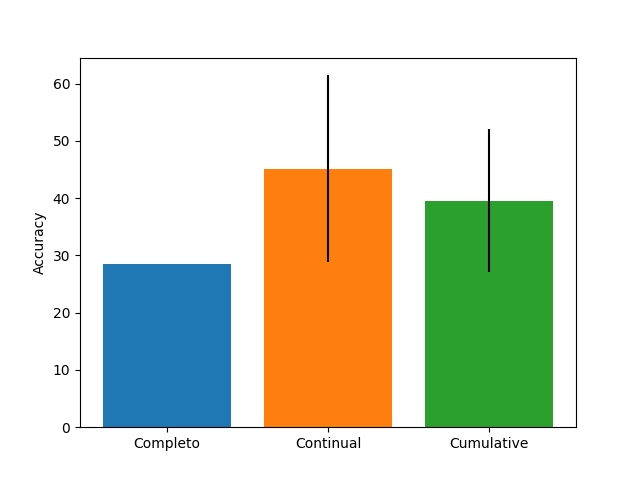
\includegraphics[scale=0.75]{img/first.png}
    \caption{Accuracy nel primo test}
    \label{fig:first}
\end{figure}
\subsection{Secondo test}
\paragraph{Modello} Il modello è simile al precedente ma con due layer GRU da 30 unità: questo è il risultato di una gridsearch.
\paragraph{Risultati} Di seguito\\
\begin{tabular}{l|c|c|c|c}
    \textbf{Scenario} & \textbf{Media epoche} & \textbf{Std. Dev.} & \textbf{Media Accuracy} & \textbf{Std. Dev} \\
    \hline 
    \textbf{Offline} & 100 & 0 & 30.36\% & 0 \\
    \textbf{Continual} & 100 & 0 & \textbf{46.17\%} & 12.50 \\
\end{tabular}
\begin{figure}
    \centering
    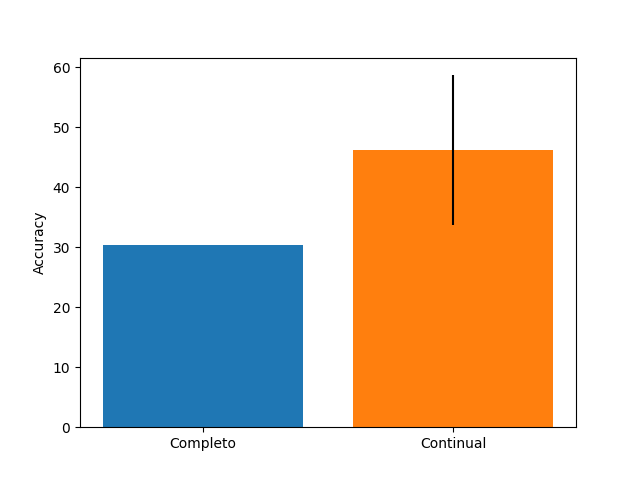
\includegraphics[scale=0.75]{img/second.png}
    \caption{Accuracy nel secondo test}
    \label{fig:second}
\end{figure}
Notando un'accuracy del 100\% sia su training set che su validation set, ho giudicato il modello inadatto per overfitting. Ho quindi deciso di cambiare dataset, prendendo tutte le istanze di ogni label.
\paragraph{Risultati} Con il nuovo dataset più capiente ho ottenuto risultati migliori\\
\begin{tabular}{l|c|c|c|c}
    \textbf{Scenario} & \textbf{Media epoche} & \textbf{Std. Dev.} & \textbf{Media Accuracy} & \textbf{Std. Dev} \\
    \hline 
    \textbf{Offline} & 9 & 0 & \textbf{56.24\%} & 0 \\
    \textbf{Continual} & 79.29 & 35.11 & 53.72\% & 14.24\\
\end{tabular}
\begin{figure}
    \centering
    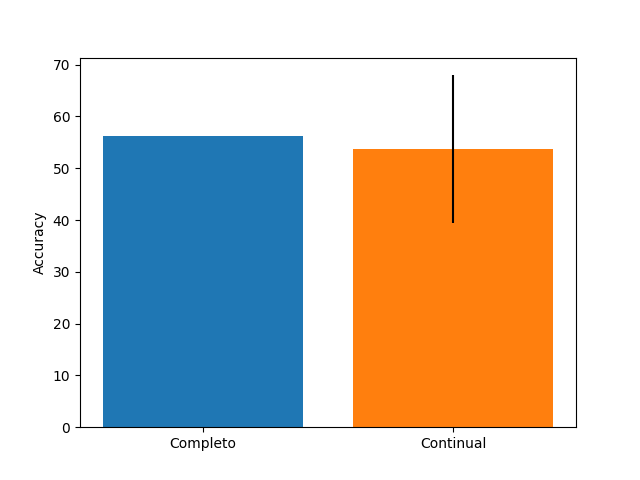
\includegraphics{\includegraphics[scale=0.75]{img/second2.png}}
    \caption{Risultati con il nuovo dataset}
    \label{fig:second2}
\end{figure}
\subsection{Terzo test}
\paragraph{Modello} Questo test l'ho eseguito sostituendo LSTM a GRU nel modello, cioè rimanendo con due layer da 30 unità più l'output layer Dense da 4 unità softmax.\\
Ho notato che un "replay" ingenuo, ovvero il portarsi dietro tutti i soggetti già usati nel training all'interno del training set successivo sommandoli con i due soggetti "nuovi", migliora di molto l'accuracy su S17. Ho quindi provato una tecnica di replay più snella: mantenere di volta in volta il 25\% casuale dei datapoint del trainingset attuale.
\paragraph{Risultati} Di seguito\\
\begin{tabular}{l|c|c|c|c}
    \textbf{Scenario} & \textbf{Media epoche} & \textbf{Std. Dev.} & \textbf{Media Accuracy} & \textbf{Std. Dev} \\
    \hline 
    \textbf{Offline} & 11 & 0 & 59.59\% & 0 \\
    \textbf{Continual} & 58.29 & 48.17 & 50.70\% & 8.24\%\\
    \textbf{Cumulative} & 26.43 & 32.20 & \textbf{62.83\%} & 8.20\%\\
    \textbf{Replay 25\%} & 17.43 & 11.32 & 61.07\% & 4.77\%\\
\end{tabular}
\begin{figure}
    \centering
    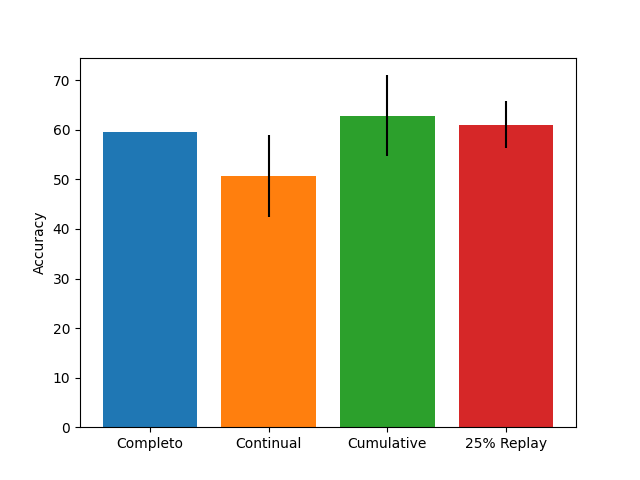
\includegraphics[scale=0.75]{img/third.png}
    \caption{Risultati nel terzo test}
    \label{fig:third}
\end{figure}
\pagebreak
\subsection{Quarto Test}
\paragraph{Scenario} A questo punto ho voluto provare una serie di modelli diversi sulla nuova tecnica, il replay training.
\paragraph{Risultati} Di seguito\\
\begin{tabular}{l|c|c|c|c}
    \textbf{Modello} & \textbf{Media epoche} & \textbf{Std. Dev.} & \textbf{Media Accuracy} & \textbf{Std. Dev} \\
    \hline 
    \textbf{Un layer LSTM con 30 unità} & 11.71 & 6.13 & \textbf{70.59\%} & 12.17\% \\
    \textbf{Un layer LSTM con 29 unità} & 12 & 10 & 52.33\% & 6.14\%\\
    \textbf{Un layer LSTM con 25 unità} & 21 & 8.59 & 58.72\% & 4.14\%\\
    \textbf{Un layer LSTM con 15 unità} & 28.14 & 24.03 & 59.88\% & 3.44\%\\
\end{tabular}
\begin{figure}
    \centering
    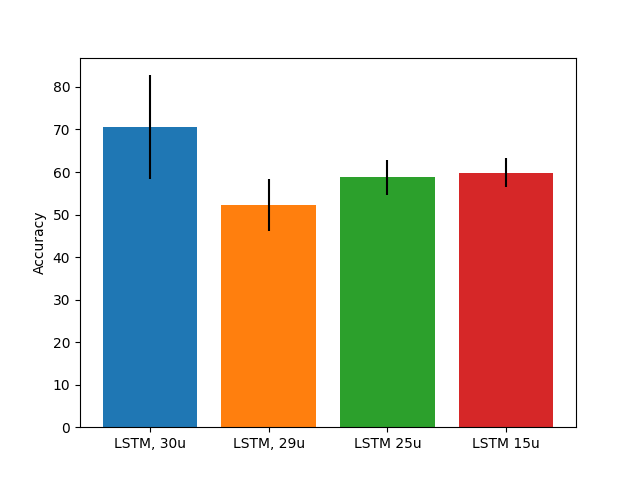
\includegraphics[scale=0.75]{img/fourth.png}
    \caption{Confronto fra modelli LSTM}
    \label{fig:fourth}
\end{figure}

\subsection{Quinto test}
\paragraph{Scenario} Stesso cambio di modello ma con GRU
\paragraph{Risultati} Di seguito\\
\begin{tabular}{l|c|c|c|c}
    \textbf{Modello} & \textbf{Media epoche} & \textbf{Std. Dev.} & \textbf{Media Accuracy} & \textbf{Std. Dev} \\
    \hline 
    \textbf{Un layer GRU con 30 unità} & 49.29 & 43.05 & \textbf{59.80\%} & 3.98\% \\
    \textbf{Due layer GRU con 30 unità} & 45 & 29.44 & 59.71\% & 3.27\%\\
\end{tabular}
\begin{figure}
    \centering
    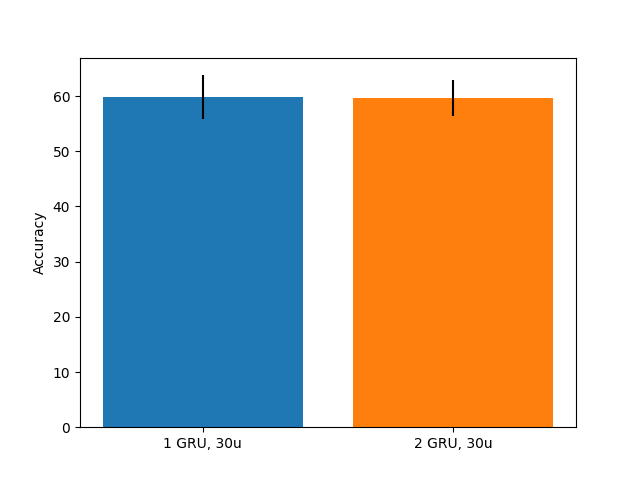
\includegraphics[scale=0.75]{img/fifth.png}
    \caption{Confronto fra modelli GRU}
    \label{fig:fifth}
\end{figure}
\subsection{Sesto Test}
\paragraph{Scenario} Ho quindi deciso di fare un test comparativo fra le varie tecniche scegliendo come modello quello da un singolo layer GRU da 30 unità.
Il test, automatizzato in un singolo script, prevede:
\begin{itemize}
    \item \textbf{total training}: soggetti S2-S16 insieme, test su S17
    \item \textbf{continual training}: soggetti S2-S3, test su S17, riprendo training con S4-S5, test e così via
    \item \textbf{cumulative training}: soggett S2-S3, test su S17, aggiungo S4-S5 al tr set, test su S17 e così via
    \item \textbf{replay training}: soggetti S2-S3, test su S17, mantengo il 25\% del tr set e aggiungo S4-S5, test e così via
\end{itemize}
\paragraph{Risultati} Di seguito\\
\begin{tabular}{l|c|c|c|c}
    \textbf{Scenario} & \textbf{Media epoche} & \textbf{Std. Dev.} & \textbf{Media Accuracy} & \textbf{Std. Dev} \\
    \hline 
    \textbf{Offline} & 14 & 0 & 65.35\% & 0\% \\
    \textbf{Continual} & 72.29 & 43.83 & 52.57\% & 8.51\%\\
    \textbf{Cumulative} & 18.71 & 33.32 & 59.18\% & 2.16\%\\
    \textbf{Replay} & 35.71 & 41.13 & \textbf{65.13\%} & 8.74\%\\
\end{tabular}
\begin{figure}
    \centering
    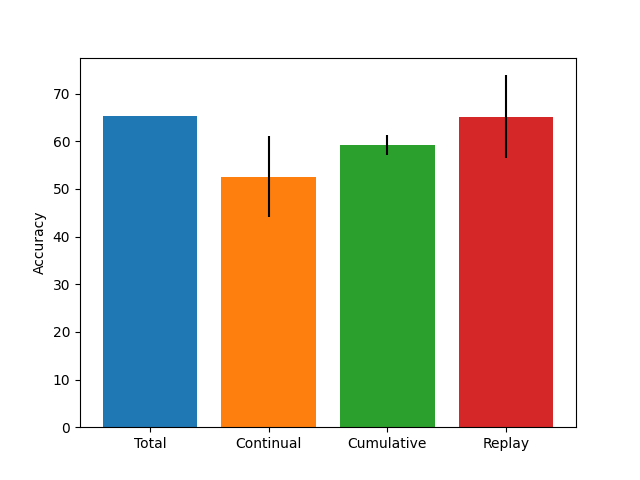
\includegraphics[scale=0.75]{img/sixth.png}
    \caption{Confronto fra scenari}
    \label{fig:sixth}
\end{figure}
Ulteriore conferma di un risultato teorico: mantenere esempi già addestrati mitiga il catastrophic forgetting.\\\\
Nel caso del continual training senza ripetizioni, si ha una costante diminuzione dell'accuracy su S17 che è sintomo di catastrophic forgetting.\\
\begin{figure}
    \centering
    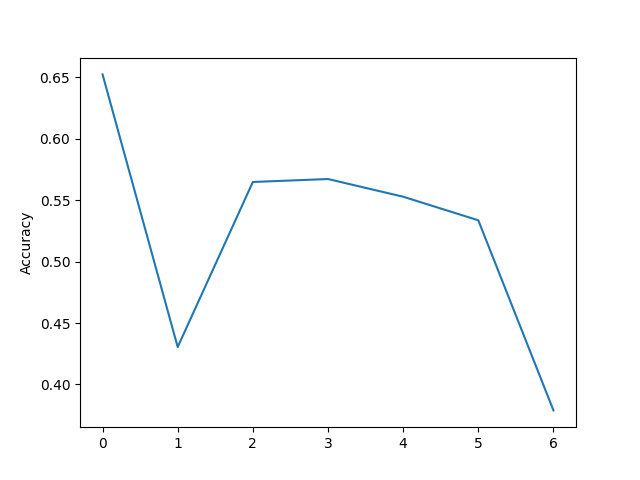
\includegraphics[scale=0.5]{img/cont6.png}
    \caption{Andamento accuracy del continual learning}
    \label{fig:cont6}
\end{figure}
Mentre il cumulative training suppongo vada in overfitting per i troppi dati.\\
\begin{figure}
    \centering
    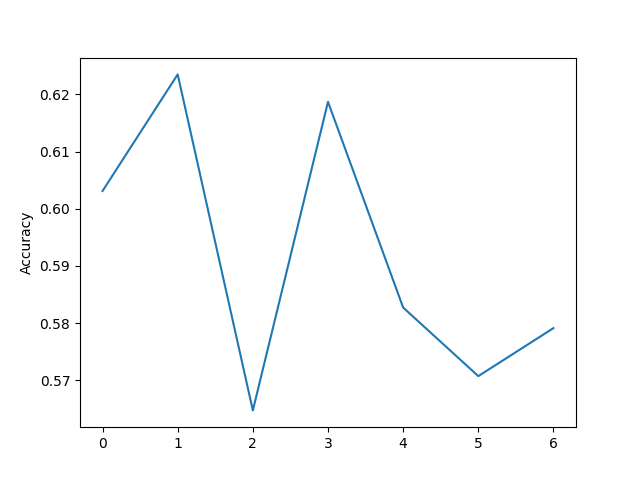
\includegraphics[scale=0.5]{img/sum6.png}
    \caption{Andamento accuracy del cumulative learning}
    \label{fig:sum6}
\end{figure}
Replay, d'altro canto, si comporta al pari del total training, pur mantenendo di coppia in coppia solo il 25\% dei dati dei soggetti precedenti.\\
\begin{figure}
    \centering
    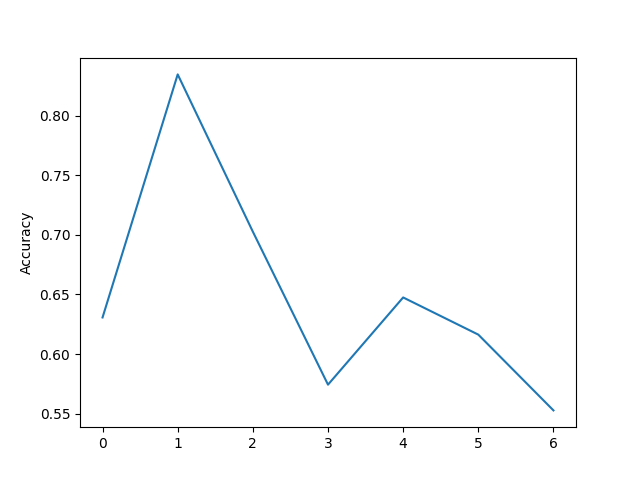
\includegraphics[scale=0.5]{img/repl6.png}
    \caption{Andamento accuracy del replay learning}
    \label{fig:repl6}
\end{figure}
\subsection{Settimo test}
\paragraph{Scenario} Vedendo come si comporta bene il replay, ho deciso di provare diverse tecniche di replay. Il modello è un layer singolo GRU da 30 unità, più quello output solito.
\begin{itemize}
    \item[] \textbf{Baseline}: tecnica usata fin'ora ma mantenendo solo il 10\% dei dati
    \item[] \textbf{25\%}: cioè mantengo il 25\% dei dati
    \item[] \textbf{Memoria episodica}, mantenendo $m = 50$ istanze a caso per ogni label
    \item[] \textbf{Memoria episodica}, mantenendo $m = 50$ \textit{predizioni} per ogni label
\end{itemize}
\paragraph{Risultati} Di seguito\\
\begin{tabular}{l|c|c|c|c}
    \textbf{Scenario} & \textbf{Media epoche} & \textbf{Std. Dev.} & \textbf{Media Accuracy} & \textbf{Std. Dev} \\
    \hline 
    \textbf{Replay 10\%} & 58.43 & 35.66 & 51.54\% & 8.53\% \\
    \textbf{Replay 25\%} & 42.71 & 39.88 & 55.69\% & 8.12\%\\
    \textbf{$m = 50$ istanze} & 45.43 & 41.74 & 56.46\% & 4.44\%\\
    \textbf{$m = 50$ previsioni} & 23 & 32.16 & \textbf{57.01\%} & 6.02\%\\
\end{tabular}
\begin{figure}
    \centering
    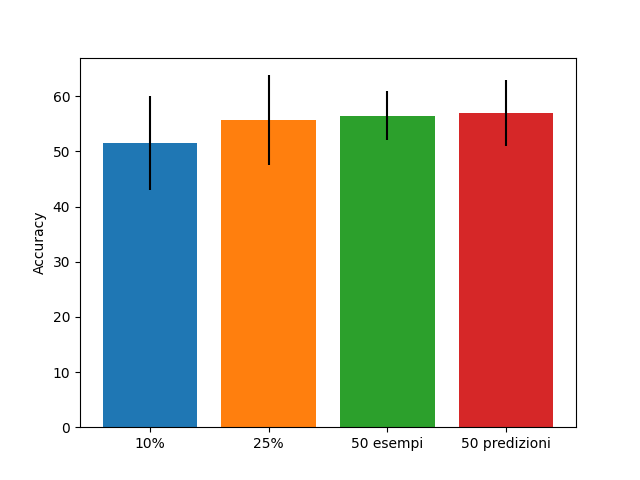
\includegraphics[scale=0.75]{img/seventh.png}
    \caption{Confronto tecniche su GRU}
    \label{fig:seventh}
\end{figure}
\subsection{Ottavo test}
\paragraph{Scenario} Stesso scenario precedente ma il modello è un layer singolo LSTM da 30 unità, più quello output solito.
\paragraph{Risultati} Di seguito\\
\begin{tabular}{l|c|c|c|c}
    \textbf{Scenario} & \textbf{Media epoche} & \textbf{Std. Dev.} & \textbf{Media Accuracy} & \textbf{Std. Dev} \\
    \hline 
    \textbf{Replay 10\%} & 26.71 & 25.63 & 53.25\% & 9.55\% \\
    \textbf{Replay 25\%} & 51.71 & 40.31 & 61.34\% & 7.22\%\\
    \textbf{$m = 50$ istanze} & 24 & 17.74 & \textbf{62.63\%} & 8.44\%\\
    \textbf{$m = 50$ previsioni} & 40.43 & 34.50 & 54.40\% & 7.44\%\\
\end{tabular}
\begin{figure}[h]
    \centering
    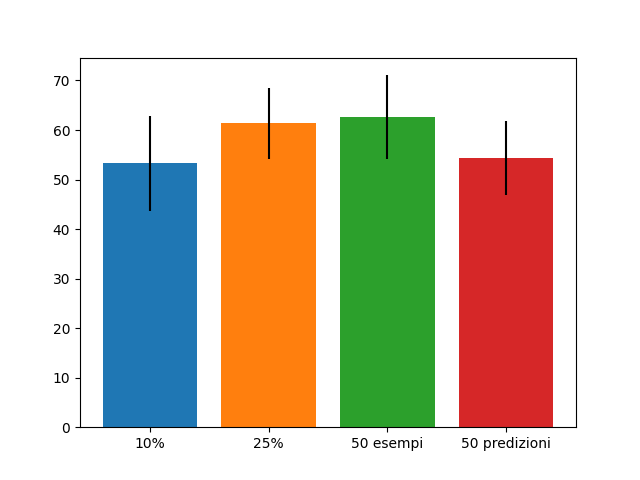
\includegraphics[scale=0.75]{img/eigth.png}
    \caption{Confronto tecniche su LSTM}
    \label{fig:eigth}
\end{figure}
\subsection{Nono test}
\paragraph{Scenario} Questa volta volevo confrontare l'uso di un modello con LSTM e l'uso di un modello con GRU, entrambi con un layer del rispettivo tipo con 30 unità e il solito layer output Dense da 4 unità softmax.
\paragraph{Risultati LSTM} Di seguito\\
\begin{figure}[h]
    \centering
    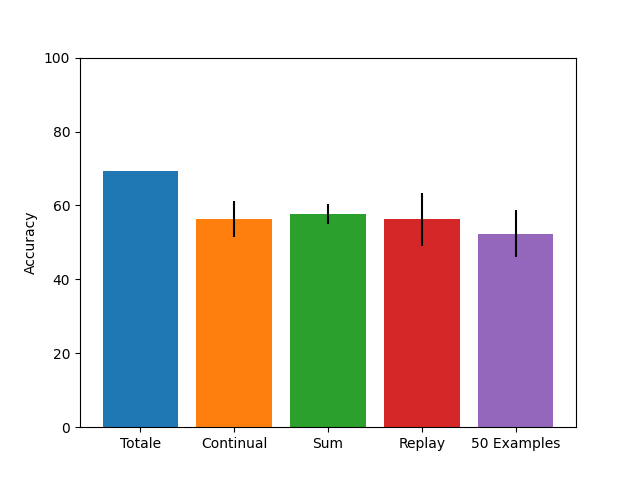
\includegraphics[scale=0.75]{img/autotest_LSTM.png}
    \caption{Risultati LSTM}
    \label{fig:autotest_LSTM}
\end{figure}
\begin{tabular}{l|c|c|c|c}
    \textbf{Scenario} & \textbf{Media epoche} & \textbf{Std. Dev.} & \textbf{Media Accuracy} & \textbf{Std. Dev} \\
    \hline 
    \textbf{Offline} & 19 & 0 &\textbf{ 59.42\%} & 0\% \\
    \textbf{Continual} & 37.43 & 33.77 & 56.35\% & 4.97\%\\
    \textbf{Cumulative} & 28.14 & 30.79 & 57.59\% & 2.60\%\\
    \textbf{Replay 25\%} & 19.43 & 16.92 & 56.22\% & 6.32\%\\
    \textbf{$m = 50$ istanze} & 20.71 & 32.69 & 52.33\% & 6.32\%\\
\end{tabular}
\paragraph{Risultati GRU} Di seguito\\
\begin{figure}[h]
    \centering
    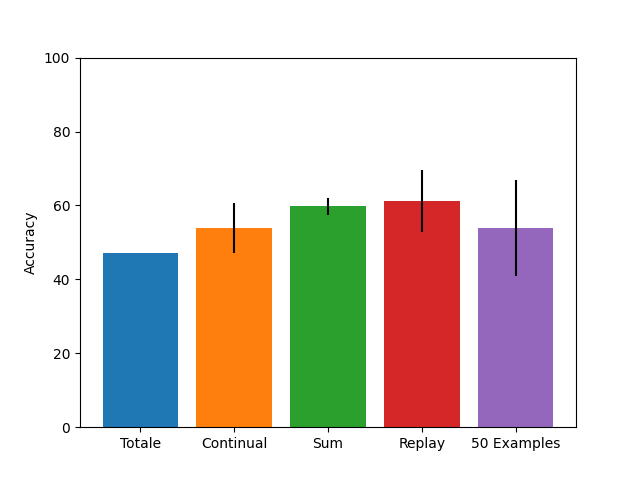
\includegraphics[scale=0.75]{img/autotest_GRU.png}
    \caption{Risultati GRU}
    \label{fig:autotest_GRU1}
\end{figure}
\begin{tabular}{l|c|c|c|c}
    \textbf{Scenario} & \textbf{Media epoche} & \textbf{Std. Dev.} & \textbf{Media Accuracy} & \textbf{Std. Dev} \\
    \hline 
    \textbf{Offline} & 16 & 0 & 47.24\% & 0\% \\
    \textbf{Continual} & 86.14 & 33.94 & 53.80\% & 6.77\%\\
    \textbf{Cumulative} & 27.43 & 33.12 & 59.75\% & 2.35\%\\
    \textbf{Replay 25\%} & 39.14 & 34.27 & \textbf{61.24\%} & 8.33\%\\
    \textbf{$m = 50$ istanze} & 41.14 & 37.23 & 53.91\% & 13.10\%\\
\end{tabular}
Le strategie "continual" si comportano meglio con GRU, mentre LSTM funziona meglio sul training offline.

\subsection{Decimo test}
\paragraph{Scenario} Ho provato il modello da 1 layer GRU da 30 unità con diversi valori di $m$ sul replay episodico
\paragraph{Risultati} Di seguito\\
\begin{figure}[h]
    \centering
    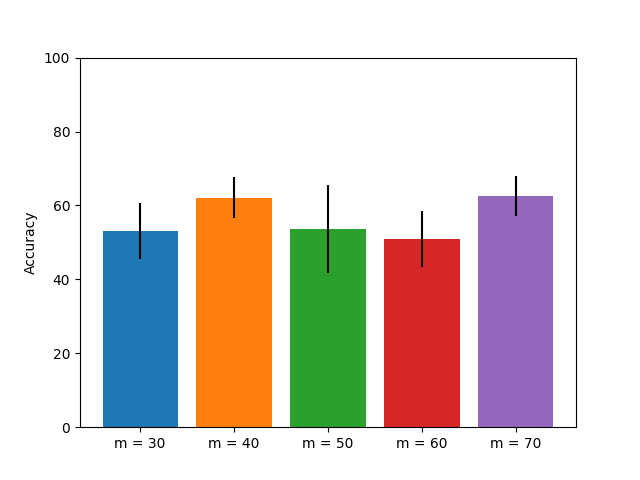
\includegraphics[scale=0.75]{img/episodic_m_test.png}
    \caption{Risultati}
    \label{fig:episodic_m_test}
\end{figure}
\begin{tabular}{l|c|c|c|c}
    \textbf{$m =$} & \textbf{Media epoche} & \textbf{Std. Dev.} & \textbf{Media Accuracy} & \textbf{Std. Dev} \\
    \hline 
    \textbf{30} & 54 & 40.07 & 53.17\% & 7.57\% \\
    \textbf{40} & 61.14 & 44.20 & 62.09\% & 5.60\%\\
    \textbf{50} & 39.14 & 42.80 & 53.61\% & 11.98\%\\
    \textbf{60} & 66.57 & 33.91 & 50.91\% & 7.57\%\\
    \textbf{70} & 43.14 & 40.35 & \textbf{62.56\%} & 5.43\%\\
\end{tabular}
\pagebreak
\subsection{Undicesimo test}
\paragraph{Obiettivo} Vorrei provare a inquadrare metriche utili a comparare i vari approcci al continual learning, in particolare poter misurare il catastrophic forgetting e il backward/forward transfer. Ho trovato, nel paper che descrive l'approccio Gradient Episodic Memory, tre metriche utili:
\begin{itemize}
    \item[\textbf{ACC}] Average accuracy = $\frac{1}{T}\sum_{i=1}^T R_{T,i}$\\
    Con questa matrica si misura l'accuratezza generale del modello.
    \item[\textbf{BWT}] Backward transfer = $\frac{1}{T-1}\sum_{i=1}^{T-1} R_{T,i} - R_{i,i}$\\
    Viene misurato l'impatto che l'apprendimento ha avuto su tutti i task precedenti.
    \item[\textbf{FWT}] Forward transfer = $\frac{1}{T-1}\sum_{i=2}^T R_{i-1,i} - b_i$\\
    Viene misurato quanto è migliorato l'apprendimento sul finale rispetto all'inizializzazione casuale iniziale.
\end{itemize}
Dove con $T$ indichiamo il numero di task, $R \in R^{T\times T}$ è la matrice delle accuratezze: dopo che il modello ha appreso il task $t_i$, valutiamo la sua performance su tutti i $T$ task. Quindi $R_{i,j}$ è la performance del modello sul task $t_j$ dopo aver osservato l'ultima istanza del task $t_i$.\\
$b$ è il vettore delle accuratezze per ogni task all'inizializzazione casuale.
\paragraph{Implementazione} Ho implementato seguendo questa filosofia: ogni classe è un "task", e a fine apprendimento su una coppia si aggiorna $R$ in base .\\
Ho quindi innanzitutto diviso il test set per task:
\begin{lstlisting}[language = Python]
Xts = pickle.load(open("WESAD/splitted/XS17_disarli.pkl", 'rb'), encoding='latin1')
yts = pickle.load(open("WESAD/splitted/yS17_disarli.pkl", 'rb'), encoding='latin1')

Xts_1, Xts_2, Xts_3, Xts_4, yts_1, yts_2, yts_3, yts_4 =
    [], [], [], [], [], [], [], []
idx_1 = [i for i, x in enumerate(yts) if x[0] == 1]
for i in idx_1:
    Xts_1.append(Xts[i])
    yts_1.append([1., 0., 0., 0.])
Xts_1, yts_1 = np.array(Xts_1), np.array(yts_1)
# ...
idx_4 = [i for i, x in enumerate(yts) if x[3] == 1]
for i in idx_4:
    Xts_4.append(Xts[i])
    yts_4.append([0., 0., 0., 1.])
Xts_4, yts_4 = np.array(Xts_4), np.array(yts_4)
\end{lstlisting}
\pagebreak
Subito dopo aver compilato il modello, preparo le metriche e inizializzo $b$:
\begin{lstlisting}[language = Python]
R = []
T = 4
b = [model.evaluate(Xts_1, yts_1)[1],
     model.evaluate(Xts_2, yts_2)[1],
     model.evaluate(Xts_3, yts_3)[1],
     model.evaluate(Xts_4, yts_4)[1]]
ACC, BWT, FWT = 0, 0, 0
\end{lstlisting}
Durante l'apprendimento, oltre a valutare sul test set intero popolo anche $R$:
\begin{lstlisting}[language = Python]
R.append([model.evaluate(Xts_1, yts_1)[1],
          model.evaluate(Xts_2, yts_2)[1],
          model.evaluate(Xts_3, yts_3)[1],
          model.evaluate(Xts_4, yts_4)[1]])
\end{lstlisting}
A fine allenamento calcolo le metriche finali (codice temporaneo):
\begin{lstlisting}[language = Python]
t = 0
for i in range(T):
        t += R[T-1][i]
ACC = t/T

t = 0
for i in range(T-1):
        t += (R[T-1][i] - R[i][i])
BWT = t/(T-1)

t = 0
for i in range(1, T):
        t += (R[i-1][i] - b[i])
FWT = t/(T-1)
\end{lstlisting}
\pagebreak
\paragraph{Risultati} Ho provato le metriche su tre scenari di continual learning diversi:
\begin{tabular}{l|c|c|c|c|c}
    \textbf{Scenario} & \textbf{Epoche} & \textbf{Accuracy} & \textbf{ACC} & \textbf{BWT} & \textbf{FWT} \\
    \hline 
    \textbf{$m = 70$} & 20.29$\pm$16.21 & 59.82\%$\pm$5.95\% & 0.4665 & -0.0202 & 0.4069 \\
    \textbf{Replay 10\%} & 46.14$\pm$42.93 & 59.58\%$\pm$13.83\% & 0.4745 & -0.1617 & 0.5320\\
    \textbf{Continual} & 48.29$\pm$37.38 & 46.44\%$\pm$11.35\% & 0.4813 & -0.0242 & 0.0481\\
\end{tabular}\\\\
L'approccio episodic (cioè replay di un numero $m$ di memorie per ogni classe/task) e quello replay (cioè replay di una percentuale del training set) hanno accuratezza sul test set sempre molto comparabili, se non adirittura simili, ma con queste ultime metriche si nota come il replay abbia durante l'apprendimento un impatto molto più grande sia sul backward transfer che sul forward transfer.\\
BWT negativo in tutti e tre i casi, ma in particolare modo nel replay, indica l'influenza negativa che si ha in generale sui task precedenti all'apprendimento di un nuovo task (cioè un elevato catastrophic forgetting).\\
FWT positivo invece indica l'influenza positiva che apprendere un task corrente ha sulla performance dei futuri task. In particolare, un FWT alto indica la capacità del modello di effettuare un apprendimento "zero-shot", cioè di apprendere un task successivo semplicemente sfruttando la struttura dei task già appresi (ed è il caso del test effettuato, avendo ad ogni passo coppie di soggetti dove sono presenti tutti i task da apprendere che quindi influenzano positivamente l'apprendimento sulle coppie successive).\\
\begin{figure}[h]
    \centering
    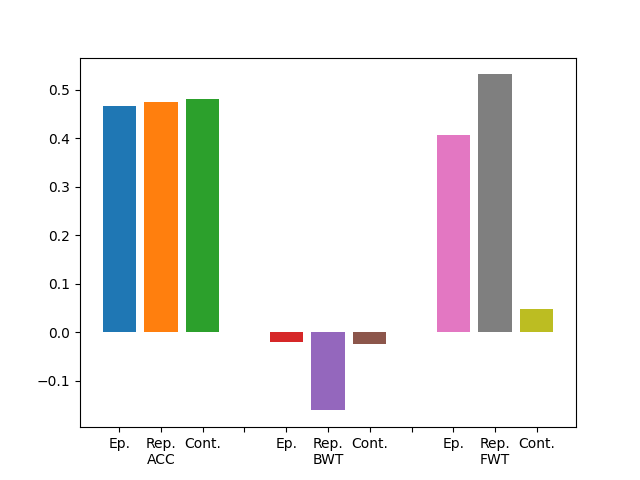
\includegraphics[scale=0.75]{img/accbwtfwt.png}
    \caption{Risultati}
    \label{fig:accbwtfwt}
\end{figure}
\begin{figure}[h]
    \centering
    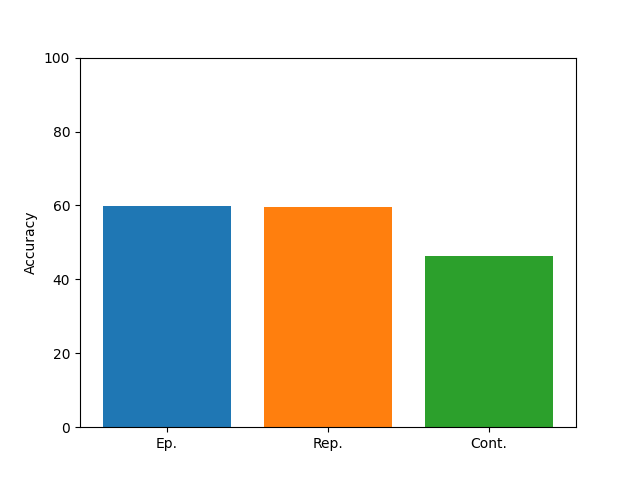
\includegraphics[scale=0.75]{img/accbwtfwt_accuracy.png}
    \caption{Accuracy}
    \label{fig:accbwtfwt_accuracy}
\end{figure}
\subsection{Dodicesimo test}
\paragraph{Obiettivo} Vedere come si comportano i vari approcci visti fin'ora ma su un modello che impara un task per volta, invece che a coppie di soggetti con tutti i task. Il test verrà fatto sempre su S17. Per prima cosa dividerò il dataset per classe, anziché per soggetto.\\
In futuro vorrei provare altri modelli, altre tecniche di replay.
\paragraph{Risultati} Di seguito i risultati raccolti
\begin{figure}[h]
    \centering
    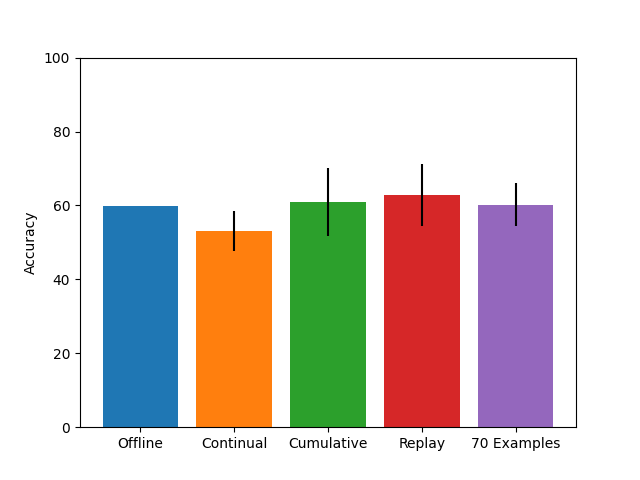
\includegraphics[scale=0.75]{img/autotest_20210701/autotest_GRU.png}
    \caption{Learning a coppia di soggetti}
    \label{fig:autotest_GRU}
\end{figure}
\begin{figure}[h]
    \centering
    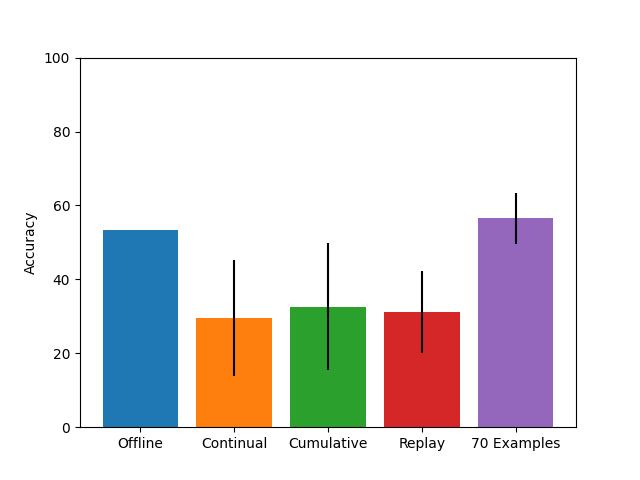
\includegraphics[scale=0.75]{img/autotest_20210701/autotest_task_GRU.png}
    \caption{Learning task per task}
    \label{fig:autotest_task_GRU}
\end{figure}
\begin{figure}[h]
    \centering
    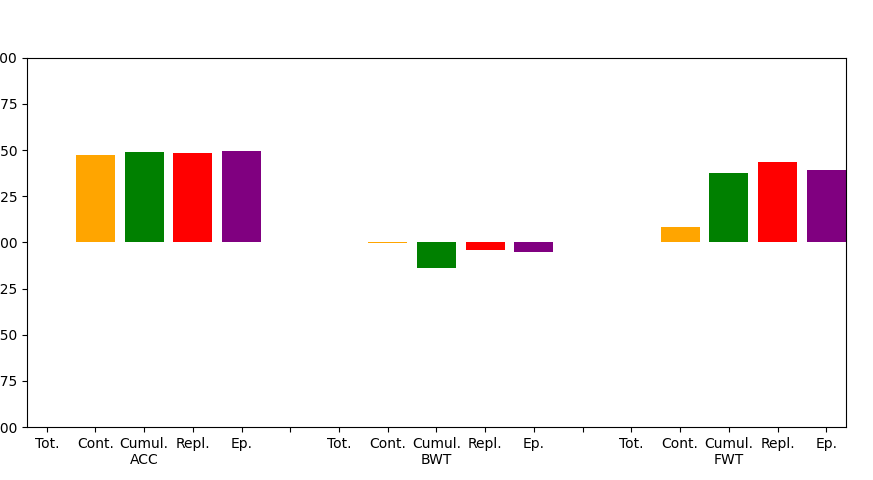
\includegraphics[scale=0.6]{img/autotest_20210701/autotest_GRU_accbwtfwt.png}
    \caption{Metriche a coppia di soggetti}
    \label{fig:autotest_GRU_accbwtfwt}
\end{figure}
\begin{figure}[h]
    \centering
    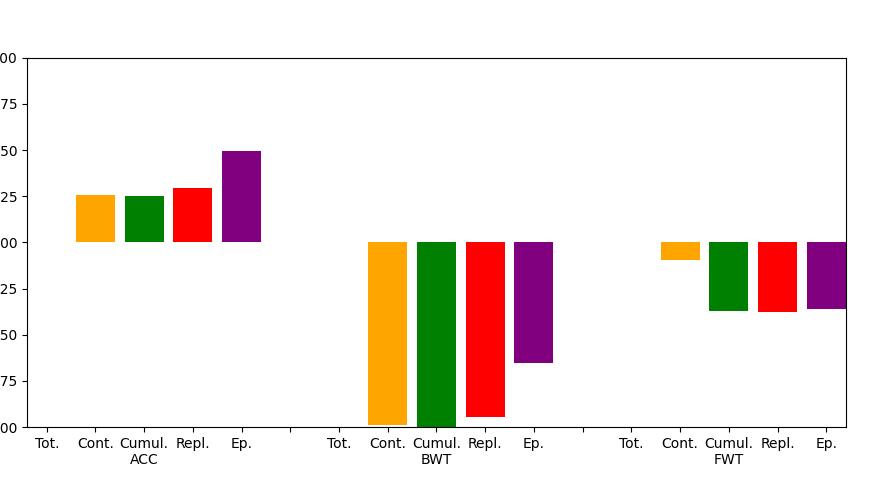
\includegraphics[scale=0.6]{img/autotest_20210701/autotest_task_GRU_accbwtfwt.png}
    \caption{Metriche task per task}
    \label{fig:autotest_task_GRU}
\end{figure}
\paragraph{Learning task per task} Di seguito\\
\begin{tabular}{l|c|c|c|c|c}
    \textbf{Scenario} & \textbf{Epoche} & \textbf{Accuracy} & \textbf{ACC} & \textbf{BWT} & \textbf{FWT} \\
    \hline 
    \textbf{Offline} & 18 & 53.24\% & - & - & - \\
    \textbf{Continual} & 99.25$\pm$1.3 & 26.47\%$\pm$15.68\% & 0.2570 & -0.9907 & -0.0935\\
    \textbf{Cumulative} & 99.25$\pm$1.3 & 32.64\%$\pm$17.07\% & 0.2507 & -0.9991 & -0.3695\\
    \textbf{Replay 25\%} & 99$\pm$1.73 & 31.24\%$\pm$11.05\% & 0.2918 & -0.9443 & -0.3756\\
    \textbf{$m = 70$} & 39.5$\pm$36.13 & \textbf{56.49\%$\pm$6.93\%} & 0.4938 & -0.6509 & -0.3595\\
\end{tabular}
\paragraph{Learning a coppie} Di seguito\\
\begin{tabular}{l|c|c|c|c|c}
    \textbf{Scenario} & \textbf{Epoche} & \textbf{Accuracy} & \textbf{ACC} & \textbf{BWT} & \textbf{FWT} \\
    \hline 
    \textbf{Offline} & 13 & 59.95\% & - & - & - \\
    \textbf{Continual} & 70$\pm$37.04 & 52.96\%$\pm$5.41\% & 0.4712 & -0.0042 & 0.0844\\
    \textbf{Cumulative} & 24.71$\pm$27.54 & 60.88\%$\pm$9.13\% & 0.4831 & -0.1369 & 0.3752\\
    \textbf{Replay 25\%} & 49.14$\pm$35.97 & \textbf{62.80\%$\pm$8.36\%} & 0.4942 & -0.0502 & 0.3903\\
    \textbf{$m = 70$} & 56.29$\pm$35.27 & 60.24\%$\pm$5.72\% & 0.4942 & -0.0502 & 0.3903\\
\end{tabular}
\subsection{Un po' di somme}
Partendo da un layer GRU da 29 unità seguito da un layer output Dense da 4 unità softmax, ho innanzitutto provato tre tecniche:
\begin{itemize}
    \item Total training: tutti i soggetti (escluso S17) sono stati uniti in un unico dataset e il modello è stato addestrato offline e testato su S17.
    \item Continual training: i soggetti sono stati divisi a coppie, escluso S17, e il modello è stato addestrato coppia per coppia testando su S17 dopo ogni coppia.
    \item Cumulative training: il training è stato eseguito coppia per coppia, ma le coppie precedentemente usate sono state mantenute anche nei training set successivi (quindi a con l'ultima coppia il training set equivaleva al dataset completo escluso S17)
\end{itemize}
Ho poi provato un modello con due layer GRU da 30 unità e un layer output Dense da 4 unità softmax sui primi due scenari di training, ottenendo fondamentalmente gli stessi risultati. Temendo overfitting, ho rifatto il dataset prendendo tutti i datapoint di ogni soggetto invece che solo una parte. Con quest'ultimo modello, sul dataset nuovo, ho ottenuto risultati migliori raggiungendo un 56\% di accuratezza sul training offline e un 53\% su quello continual.

Quindi ho provato un modello con due layer LSTM da 30 unità e un layer output Dense da 4 unità softmax, ottenendo risultati ancora migliori sui tre scenari. Ho aggiunto un nuovo scenario:
\begin{itemize}
    \item Replay training: dopo aver usato una coppia, ne mantengo il 25\% (default) dai dati da usare nel training assieme alla coppia successiva. Fornisce risultati a metà strada tra il continual e il cumulative.
\end{itemize}

Con la nuova tecnica, ho provato diversi modelli sia GRU che LSTM con un numero di unità tra i 30 e i 15. Ho concluso che il modello con un singolo layer LSTM da 30 unità e quello con un singolo layer GRU da 30 unità sono i migliori, procedendo a comparare le varie tecniche sul singolo layer GRU. Ottengo un comportamento del replay al 25\% comparabile al training offline, seppur oscillante tra l'85\% e il 55\% (con l'offline che si attesta sul 65\%). Il cumulative è molto più stabile, intorno al 60\% con una deviazione standard del 2\%.

Giudicando ottime le tecniche di replay, ne ho provate diverse:
\begin{itemize}
    \item Replay 10\%
    \item Replay 25\%
    \item Episodica  $m=50$  istanze
    \item Episodica  $m=50$  predizioni
\end{itemize}

Con il replay al 25\% e l'episodico sulle istanze con i comportamenti migliori. Ho provato anche con un layer LSTM da 30 unità e un layer output Dense da 4 unità softmax, ottenendo risultati simili ma migliori.

Ho confrontato i due modelli, ottenendo un risultato migliore su LSTM per il training offline, mentre le strategie continual si comportano meglio con GRU. Va però in contrasto con quanto osservato fin'ora.

Confrontando vari valori di  $m$, ho trovato in  $m=70$  il comportamento migliore. Andrebbe fatta un'altra ricerca in quell'intorno, magari tra 60 e 100.

Successivamente ho studiato diverse metriche (ACC, BWT e FWT) che confermano l'episodic come la tecnica migliore: finendo con un'ACC comparabile al replay al 10\%, ha però un catastrophic forgetting di quasi 10 volte inferiore.

Ho anche comparato l'apprendere task per task invece che coppia per coppia, ottenendo però accuratezze molto basse su continual, cumulative e replay, nonostante l'offline (dove il dataset non cambia) e l'episodic mantengano grossomodo le stesse capacità.

\begin{figure}[h]
    \centering
    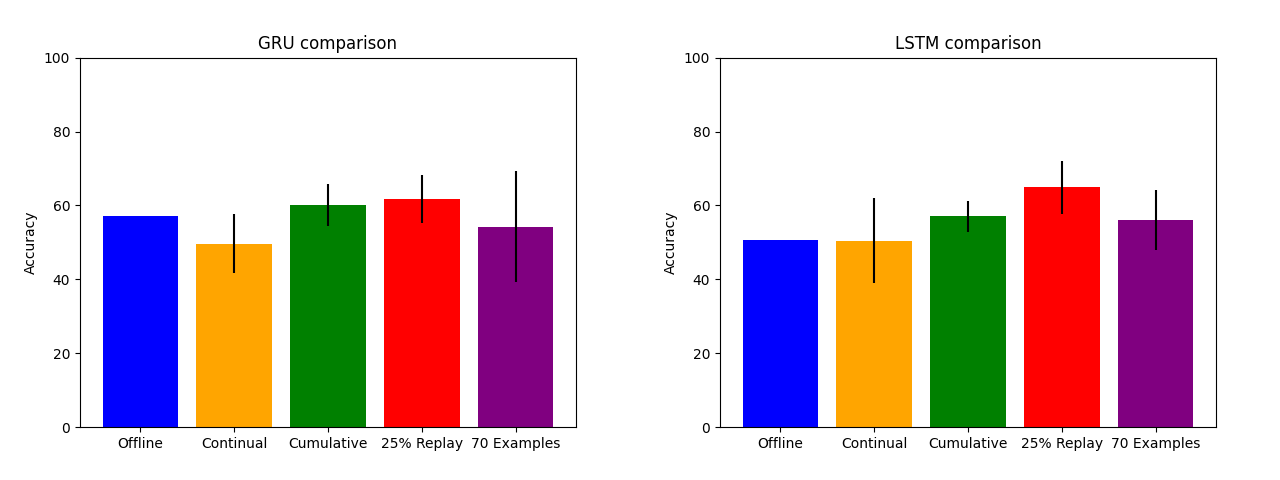
\includegraphics[scale=0.5]{img/autotestv.png}
    \caption{Comparazione fra modelli}
    \label{fig:autotest_comparison}
\end{figure}

\begin{figure}[h]
    \centering
    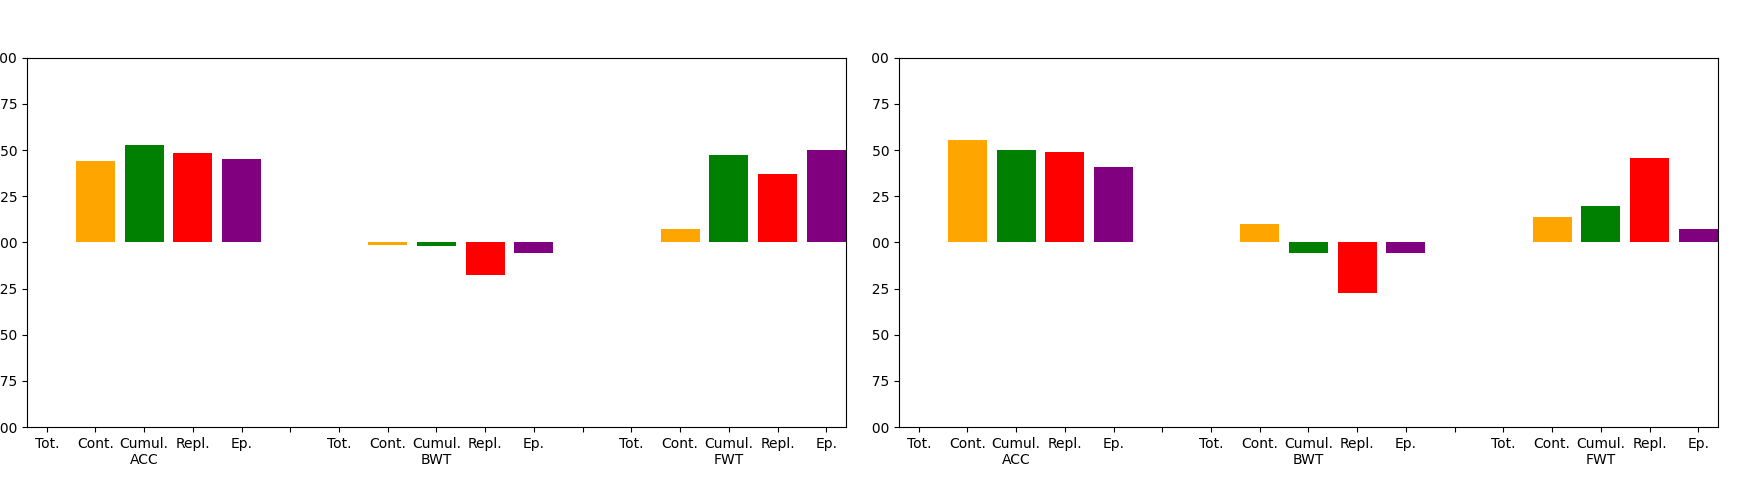
\includegraphics[scale=0.33]{img/autotestv_accbwtfwt.png}
    \caption{Comparazione fra modelli}
    \label{fig:autotest_comparison_metrics}
\end{figure}
\subsection{Tredicesimo test}
\paragraph{Generative replay} Ho valutato l'idea di creare un modello generativo per poter eseguire l'episodic training senza dover memorizzare i dati. L'idea che ho realizzato è molto semplice: allenare un modello "al contrario", cioè passandogli i label come input e aspettandomi come output le 14 features del dataset WESAD. L'ho realizzato con il seguente modello:
\begin{lstlisting}[language = Python]
model = tf.keras.models.Sequential()
model.add(tf.keras.layers.Dense(30))
model.add(tf.keras.layers.Dense(14,
                  kernel_regularizer = tf.keras.regularizers.l1_l2(l1 = 1e-6, l2 = 1e-6),
                  bias_regularizer = tf.keras.regularizers.l1_l2(l1 = 1e-4, l2 = 1e-4),
                  activity_regularizer = tf.keras.regularizers.l1_l2(l1 = 1e-4, l2 = 1e-4)))
opt = tf.keras.optimizers.Adam(learning_rate = 0.005, beta_1 = 0.85, beta_2 = 0.999)
model.compile(loss = 'mse', optimizer = opt)
\end{lstlisting}
Allenandolo sul dataset con batch da 512 elementi. Testandolo su S17 la loss è 0.9588 e testandolo velocemente, generando delle sequenze da 100 elementi per ogni classe, i risultati sono buoni:
\begin{lstlisting}[language = Python]
generator = tf.keras.models.load_model('wesad_generative.h5')
classificator = tf.keras.models.load_model('episodicGRU')
first, second, third, fourth = [], [], [], []
for i in range(100):
    first.append(generator.predict(np.array([[1., 0., 0., 0.]]))[0])
    second.append(generator.predict(np.array([[0., 1., 0., 0.]]))[0])
    third.append(generator.predict(np.array([[0., 0., 1., 0.]]))[0])
    fourth.append(generator.predict(np.array([[0., 0., 0., 1.]]))[0])

first = np.array(first).reshape(-1, 100, 14)
second = np.array(second).reshape(-1, 100, 14)
third = np.array(third).reshape(-1, 100, 14)
fourth = np.array(fourth).reshape(-1, 100, 14)

print(classificator.predict(first))
print(classificator.predict(second))
print(classificator.predict(third))
print(classificator.predict(fourth))
\end{lstlisting}
Output:
\begin{verbatim}
[[9.9999845e-01 5.4661302e-07 6.5005071e-07 2.8123785e-07]]
[[9.4253558e-08 9.9999928e-01 1.1999366e-07 4.3563784e-07]]
[[1.9276902e-06 1.3294758e-07 9.9997914e-01 1.8861941e-05]]
[[1.3735850e-07 1.3718072e-07 7.1482100e-07 9.9999905e-01]]
\end{verbatim}
Che dimostra come la generazione e il riconoscimento siano quantomeno sulla "stessa linea d'onda".
\paragraph{Scenario} Ho quindi prodotto uno script che ricalca quello dell'episodic learning ma genera $m$ sottosequenze invece di salvarne $m$ casuali dal dataset.\\
Provo due casi: uno dove genero i replay una sola volta, e li uso durante tutto il training, e uno dove li genero ad ogni coppia di utenti.
\paragraph{Risultati} A seconda di quando genero il replay set:\\
\begin{tabular}{l|c|c|c|c|c}
    \textbf{Generazione} & \textbf{Epoche} & \textbf{Accuracy} & \textbf{ACC} & \textbf{BWT} & \textbf{FWT} \\
    \hline 
    \textbf{A inizio training} & 76.29$\pm$37.95 & \textbf{55.76\%$\pm$9.56\%} & 0.5594 & -0.0482 & 0.2262 \\
    \textbf{Ad ogni coppia} & 61.14$\pm$44.95 & 52.95\%$\pm$11.34\% & 0.5646 & 0.0117 & -0.0240\\
\end{tabular}
\subsection{Quattordicesimo test}
Ho preparato il dataset ASCERTAIN e ho provato diversi modelli per selezionare quello con le performance migliori.
\paragraph{Risultati} Di seguito:\\
\begin{tabular}{l|c|c}
    \textbf{Modello} & \textbf{Epoche} & \textbf{Accuracy} \\
    \hline 
    \textbf{GRU 2 layer 16 unità} & 8 & 35.88\% \\
    \textbf{GRU 1 layer 24 unità} & 6 & 33.46\% \\
    \textbf{GRU 2 layer 24 unità} & 4 & \textbf{39.37\%} \\
    \textbf{LSTM 1 layer 40 unità} & 4 & 34.54\% \\
    \textbf{LSTM 1 layer 38 unità} & 5 & 35.32\% \\
    \textbf{LSTM 1 layer 35 unità} & 6 & 36.09\% \\
    \textbf{LSTM 1 layer 30 unità} & 4 & 35.32\% \\
    \textbf{LSTM 1 layer 20 unità} & 7 & 35.58\% \\
\end{tabular}\\
Il risultato è stato anche confermato da una gridsearch
\pagebreak
\subsection{Risultati test}
\paragraph{WESAD} Usando come modello un layer GRU da 30 unità, su WESAD ho ottenuto i seguenti risultati:

\begin{tabular}{l|c|c|c|c|c|c|c|c}
\textbf{Scenario} & \textbf{Epoche} & \textbf{Tempo} & \textbf{Tempo tot} & \textbf{Acc.} & \textbf{ACC} & \textbf{BWT} & \textbf{FWT} & \textbf{Memoria}\\
\hline
 \textbf{Offline} & 13 & 148,01s & 148,01 s & 54,68 & - & - & - & 2.391,51 Mb\\
\textbf{Continual} & 67,00$\pm$41,98 & 436,74 s & 3.057,18 s & 62,50$\pm$11,22 & 0,5988 & 0,1074 & 0,4392 & 2.189,70 Mb\\
\textbf{Cumulative} & 26,43$\pm$30,53 & 613,79 s & 4.296,53 s & \textbf{62,69$\pm$3,99} & 0,4825 & -0,041 & 0,4653 & 2.361,97 Mb\\
\textbf{Replay 25\%} & 57,29$\pm$35,93 & 479,29 s & 3.355,03 s & 57,52$\pm$9,62 & 0,4696 & -0,0526 & 0,3516 & 2.225,91 Mb\\
\textbf{m = 70} & 37,86$\pm$35,91 & 327,58 s & 2.293,06 s & 58,43$\pm$4,50 & 0,442 & -0,0868 & 0,2336 & 2.148,99 Mb\\
\textbf{EWC} & 71,57$\pm$41,46 & 878,08 s & 6.146,56 s & 56,80$\pm$9,66 & 0,4834 & -0,1785 & 0,2417 & 2.199,43 Mb\\
\textbf{LWF} & 73,86$\pm$33,39 & 2.601,09 s & 18.207,63 s & 50,41$\pm$9,94 & 0,4692 & -0,0393 & 0,1013 & 2.154,66 Mb\\
\end{tabular}
Usando come modello un layer LSTM da 30 unità, su WESAD ho ottenuto i seguenti risultati:

\begin{tabular}{l|c|c|c|c|c|c|c|c}
\textbf{Scenario} & \textbf{Epoche} & \textbf{Tempo} & \textbf{Tempo tot} & \textbf{Acc.} & \textbf{ACC} & \textbf{BWT} & \textbf{FWT} & \textbf{Memoria}\\
\hline
 \textbf{Offline} & 28 & 228.52 s & 228.52 s & \textbf{76.86} & - & - & - & 2.397,12 Mb\\
\textbf{Continual} & 62.86$\pm$43.37 & 436.59 s & 3.056,13 s & 54.11$\pm$9.91 & 0,4857 & 0,0002 & 0,0538 & 2.216,76 Mb\\
\textbf{Cumulative} & 12.86$\pm$9.09 & 557.89 s & 3905.23 s & 62.04$\pm$5.88 & 0,4914 & -0,128 & 0,3212 & 2404,07 Mb\\
\textbf{Replay 25\%} & 15.14$\pm$7.75 & 202.12 s & 1414.84 s & 57.55$\pm$4.13 & 0,4508 & -0,0961 & 0,1767 & 2208,65 Mb\\
\textbf{m = 70} & 29.29$\pm$30.47 & 257.25 s & 1800.75 s & 57.61$\pm$5.11 & 0,4821 & -0,2283 & 0,2044 & 2.146,38 Mb\\
\textbf{EWC} & 47.14$\pm$37.03 & 753.18 s & 5272.26 s & 53.49$\pm$9.31 & 0,4745 & 0,0121 & 0,3541 & 2195,50 Mb\\
\textbf{LWF} & 46.43$\pm$32.16 & 1699.19 s & 11894.33 s & 48.89$\pm$16.21 & 0,5276 & 0.0709 & -0,0287 & 2136,14 Mb\\
\end{tabular}
\paragraph{ASCERTAIN} Usando come modello due layer GRU da 24 unità, su ASCERTAIN ho ottenuto i seguenti risultati:

\begin{tabular}{l|c|c|c|c|c|c|c|c}
\textbf{Scenario} & \textbf{Epoche} & \textbf{Tempo} & \textbf{Tempo tot} & \textbf{Acc.} & \textbf{ACC} & \textbf{BWT} & \textbf{FWT} & \textbf{Memoria}\\
\hline
 \textbf{Offline} & 13 & 1.012,01 s & 1.012,01 s & 33,59 & - & - & - & 4.136,99 Mb\\
\textbf{Continual} & 7,38$\pm$2,50 & 680,06 s & 5.440,48 s & 34,50$\pm$4,87 & 0,2262 & 0,0747 & 0,0429 & 2.648,29 Mb\\
\textbf{Cumulative} & 7,5$\pm$7,19 & 3.171,71 s & 25.373,68 s & 	32,03$\pm$2,79 & 0,2781 & -0,0264 & 0,0346 & 4.066,37 Mb\\
\textbf{Replay 25\%} & 5,12$\pm$3,14 & 778,39 s & 6.227,12 s & 33,99$\pm$4,36 & 0,202 & -0,0434 & 0,0465 & 2.732,64 Mb\\
\textbf{m = 70} & 5,12$\pm$2,71 & 647,57 s & 5.180,56 s & 35,00$\pm$4,16 & 0,2404 & 0,0569 & -0,038 & 2.815,67 Mb\\
\textbf{EWC} & 18,88$\pm$9,58 & 2.583,83 s & 20.670,64 s & \textbf{35,41$\pm$3,48} & 0,2425 & -0,0593 & 0,051 & 2.497,26 Mb\\
\textbf{LWF} & 13,88$\pm$1,54 & 2.199,38 s & 17.595,04 s & 35,21$\pm$3,83 & 0,2556 & 0,0551 & 0,0413 & 2.369,36 Mb\\
\end{tabular}
Usando come modello un layer LSTM da 35 unità, su ASCERTAIN ho ottenuto i seguenti risultati:

\begin{tabular}{l|c|c|c|c|c|c|c|c}
\textbf{Scenario} & \textbf{Epoche} & \textbf{Tempo} & \textbf{Tempo tot} & \textbf{Acc.} & \textbf{ACC} & \textbf{BWT} & \textbf{FWT} & \textbf{Memoria}\\
\hline
 \textbf{Offline} & 5 & 390.34 s & 390.34 s & \textbf{37.95} & - & - & - & 4115.21 Mb\\
\textbf{Continual} & 5.75$\pm$2.68 & 386.83 s & 3094.64 s & 34,97$\pm$4,50 & 0,2298 & 0,0677 & -0,027 & 2567.67 Mb\\
\textbf{Cumulative} & 4$\pm$2.45 & 1425.36 s & 11402.88 s & 31.15$\pm$2.54 & 0,2484 & -0,0057 & 0,0525 & 3566.31 Mb\\
\textbf{Replay 25\%} & 4.62$\pm$4.09 & 485.86 s & 3886.88 s & 34.23$\pm$4.57 & 0,207 & 0,0341 & -0,0526 & 2556.10 Mb\\
\textbf{m = 70} & 5.88$\pm$3.06 & 434.11 s & 3472.88 s & 33.70$\pm$4.02 & 0,210 & 0,0467 & 0,0103 & 2724.39 Mb\\
\textbf{EWC} & 18.88$\pm$15.02 & 1660.97 s & 13287.76 s & 33.86$\pm$4.48 & 0.2404 & 0.0608 & 0.0315 & 2551.47 Mb\\
\textbf{LWF} & 17$\pm$2.92 & 1952.19 s & 15617.52 s & 34.31$\pm$3.43 & 0.2334 & 0.0557 & 0.0017 & 2684.69 Mb\\
\end{tabular}
\section{Altre strategie}
\subsection{Elastic Weight Consolidation}
L'implementazione è stata fatta seguendo questo codice\\ \texttt{https://seanmoriarity.com/2020/10/18/continual-learning-with-ewc/}
aggiungendo un output più descrittivo, l'early stopping (con patience = 10) e adattando il training loop per essere eseguito mentre arrivano le coppie di soggetti. Il file in questione è \texttt{ewc\_train.py} al seguente link\\ \texttt{https://teaching-gitlab.di.unipi.it/f.matteoni/thesis-code/-/blob/master/ewc\_train.py}
\begin{tabular}{l|c|c|c|c|c}
    \textbf{Dataset} & \textbf{Epoche} & \textbf{Accuracy} & \textbf{ACC} & \textbf{BWT} & \textbf{FWT} \\
    \hline 
    \textbf{WESAD} & 58$\pm$43.38 & 50.13\%$\pm$12.61\% & 0.3646 & -0.195 & 0.1902\\
    \textbf{ASCERTAIN} & 28.88$\pm$14.72 & 34.70\%$\pm$3.98\% & 0,2327 & 0,0473 & -0,0206
\end{tabular}
\subsection{Learning Without Forgetting}
L'implementazione è stata realizzata seguendo il paper relativo, al link\\ \texttt{https://arxiv.org/pdf/1606.09282.pdf}. Anche qua, aggiungendo un output più descrittivo, l'early stopping (con patience = 10) e adattando il training loop per essere eseguito mentre arrivano le coppie di soggetti. Il file in questione è \texttt{lwf\_train.py} al seguente link\\ \texttt{https://teaching-gitlab.di.unipi.it/f.matteoni/thesis-code/-/blob/master/lwf\_train.py}
\begin{tabular}{l|c|c|c|c|c}
    \textbf{Dataset} & \textbf{Epoche} & \textbf{Accuracy} & \textbf{ACC} & \textbf{BWT} & \textbf{FWT} \\
    \hline 
    \textbf{WESAD} & 86.71$\pm$21.61 & 55.7\%$\pm$11.20\% & 0.5585 & 0.0722 & -0.1078\\
    \textbf{ASCERTAIN} & 13.5$\pm$1.41 & 34,77\%$\pm$4,01\%& 0,2077 & 0,0278 & -0,0316
\end{tabular}

\section{Problema nell'accuracy}
Facendo un veloce recap, fino alla call con Lomonaco di Mercoledì io usavo l’intero dataset WESAD, diviso per soggetti, mentre da Mercoledì ho provato a bilanciarlo prendendo, per ogni soggetto, 100 sequenze da 100 datapoint per ogni classe così da mitigare lo sbilanciamento delle classi. Da allora ho cercato un modello che mi garantisse un’accuracy offline apprezzabile, ma non sono mai andato sopra il 50\% (con qualche falso positivo che ha dato il 70\% circa).\\
La differenza fondamentale che ho notato rispetto al paper di riferimento (RNN for HSM) è che io uso come test set S17, poiché nello scenario continual avendo soggetto per soggetto ho pensato che il “test” più sensato sia classificare i dati del soggetto in arrivo, mentre nel paper viene usata la classica partizione del dataset comprensivo di tutti i soggetti. Così facendo, anche io riesco ad ottenere un’accuracy intorno al 95\%.\\\\
La mia conclusione è che la difficoltà sta nel classificare i dati di un solo soggetto invece di prendere dati dai soggetti precedenti. Mi spiego meglio: se uso solo S17 come soggetto di test, e il training lo eseguo sui soggetti precedenti, non riesco a classificare bene S17 perché è una persona nuova, diversa, con parametri diversi per le classi.

\paragraph{WESAD} La soluzione consiste nel creare un test set estraendo dati da ogni soggetto, e mantenere i soggetti separati senza però i dati che sono stati selezionati nel test set.\\
Così facendo, dopo un po' di prove, ottengo un modello che raggiunge il 99.40\% di accuracy sul test set "partizionato".

\paragraph{ASCERTAIN} Per ASCERTAIN ho scelto un approccio diverso: i soggetti sono stati tutti "uniti" per poi essere risuddivisi in soggetti fittizi con un migliore bilanciamento delle classi.

\subsection{Risultati finali}
\paragraph{WESAD} Usando come modello due layer GRU da 18 unità, su WESAD ho ottenuto i seguenti risultati:\\
\begin{tabular}{l|c|c|c|c|c|c|c}
\textbf{Scenario} & \textbf{Epoche} & \textbf{Tempo tot} & \textbf{Acc.} & \textbf{ACC} & \textbf{BWT} & \textbf{FWT} & \textbf{Memoria}\\
\hline
 \textbf{Offline} & 28 & 94,69 s & 99,07 & - & - & - & 2061,40 Mb\\
\textbf{Continual} & 54$\pm$38,53 & 1044,89 s & 74,09$\pm$2,05 & 0,7829 & 0,0377 & 0,4181 & 2169,16 Mb\\
\textbf{Cumulative} & 39$\pm$19,35 & 3160,43 s & 83,75$\pm$7,38 & 0,8323 & 0,0248 & 0,06989 & 2293,87 Mb\\
\textbf{Replay 25\%} & 40,14$\pm$28,26 & 1071,70 s & 78,51$\pm$6,92 & 0,8236 & 0,0483 & 0,4870 & 2184,77 Mb\\
\textbf{m = 70} & 24,43$\pm$23,27 & 817,18 s & 78,92$\pm$7,89 & 0,8912 & 0,086 & 0,3796 & 2105,37 Mb\\
\textbf{EWC} & 43,14$\pm$22,82 & 500,08 s & 71,44$\pm$5,02 & 0,7738 & 0,1154 & 0,504 & 2192,25 Mb\\
\textbf{LWF} & 40,57$\pm$14,29 & 3308,34 s & 70,27$\pm$2,99 & 0,7125 & 0,0966 & 0,4063 & 2127,07 Mb\\
\end{tabular}

\paragraph{ASCERTAIN} Usando come modello due layer GRU da 24 unità, su ASCERTAIN ho ottenuto i seguenti risultati:\\
\begin{tabular}{l|c|c|c|c|c|c|c}
\textbf{Scenario} & \textbf{Epoche} & \textbf{Tempo tot} & \textbf{Acc.} & \textbf{ACC} & \textbf{BWT} & \textbf{FWT} & \textbf{Memoria}\\
\hline
 \textbf{Offline} & 3 & 29,14 s & 42,78 & - & - & - & 1817,28 Mb\\
\textbf{Continual} & 23$\pm$13,77 & 408,48 s & 37,90$\pm$4,65 & 0,2532 & 0,0735 & -0,119 & 2166,97 Mb\\
\textbf{Cumulative} & 8,62$\pm$8,03 & 961.04 s & 38,77$\pm$4,97 & 0,2843 & -0,0362 & -0,0558 & 2293,38 Mb\\
\textbf{Replay 25\%} & 10,38$\pm$13,36 & 330 s & 39,06$\pm$4.10 & 0,2675 & 0,1315 & -0,0755 & 2172,41 Mb\\
\textbf{m = 70} & 8,88$\pm$6,21 & 446,64 s & 36,89$\pm$6,31 & 0,2844 & -0,019 & 0,2685 & 2225,02 Mb\\
\textbf{EWC} & 25,12$\pm$14,35 & 836,16 s & 36,30$\pm$4,50 & 0,2256 & -0,0309 & 0,0984 & 2168,57 Mb\\
\textbf{LWF} & 24,62$\pm$16,73 & 942 s & 37,64$\pm$5,45 & 0,2601 & 0.0837 & 0,1088 & 2113,61 Mb\\
\end{tabular}
\fi
\end{document}